% ==================================================
% CHAPTER 5 — ANALYSIS AND SPECIFICATIONS
% ==================================================

\mychapter{Implementation and Realization}

\section{Introduction}

In this chapter we describe how our platform was built and the technologies chosen for each layer of the system. Chapter~4 defined the specifications; here we focus on realization: our application, the scraping and analysis engine, and their integration through our BDD.

The implementation covers the following functional areas:

\begin{itemize}
    \item User authentication and role-based access (brand, influencer, platform administrator)
    \item Influencer discovery, lists, and live profile scanning (scraping and analysis engine)
    \item Campaign wizard, marketplace, pipeline management, and BIS matching
    \item Email outreach via brand-configured Gmail SMTP
    \item In-app campaign chat and secure token-based application and draft links
    \item Localized wallet operations (CCP, BaridiMob, DZD) with administrator validation
    \item Multilingual ML scoring and credibility analysis (scraping and analysis engine)
\end{itemize}

We begin with the general architecture, then present the technology stack, and conclude with an overview of the principal user interfaces that implement the requirements defined in the previous chapter.

\section{General Architecture}

The architecture of our platform follows a \textbf{modular two-layer design} rather than a full microservices mesh. \textbf{Our application} handles all product workflows---authentication, discovery, campaigns, chat, email configuration, and wallet management---through its internal service layer and BDD access components. The \textbf{scraping and analysis engine} handles data-intensive operations: multi-platform scraping, ML scoring, and BIS matching. Both layers share our BDD, which keeps influencer profiles, campaign state, and financial records consistent across the system.

\begin{itemize}
    \item \textbf{Presentation layer:} The user-facing layer serves three roles---brand, influencer, and platform administrator---through role-specific dashboards. Brands use discovery (filters, lists, profile side panels), the six-step campaign wizard, marketplace management, email outreach configuration, campaign pipeline views, and wallet deposit flows. Influencers browse the marketplace, manage offers, submit drafts, use campaign chat, and request CCP withdrawals. The administrator validates deposits and processes withdrawal requests. Secure token-based invitation links allow unregistered creators to enter the pipeline without prior account creation.

    \item \textbf{Application service layer:} Server-side services act as the integration boundary between the user interface and backend resources. They query our BDD, invoke the scraping and analysis engine for scraping and matching, send emails through brand-configured Gmail SMTP, and enforce role-based access. Each feature module exposes dedicated services while sharing common authentication controls.

    \item \textbf{Authentication module:} User identity is managed through our authentication module with email verification for brands, session management, and role-based access policies that restrict data access by user type. Authentication is a cross-cutting concern applied at the service and database policy layers.

    \item \textbf{Business Logic Component:}The BusinessLogic component represents the operational core of the platform. It is responsible for coordinating the main business processes, including campaign management, influencer interactions, payment processing, contract handling, and other activities related to the influencer marketing workflow. During the architectural design phase, we chose to centralize these processes within a dedicated component in order to separate business rules from infrastructure and supporting services.

A large portion of the platform's functionality depends on this component. Requests received from users are processed here before being forwarded to the appropriate services or data resources. Based on what we observed throughout the development process, concentrating business operations within a single layer improved the organization of the application and provided a clearer structure for managing interactions between the different modules. As the platform evolved and new functionalities were introduced, this component remained the primary coordination point for most operational processes.
   
    \item \textbf{Machine Learning Service (scraping and analysis engine):} The scraping and analysis engine provides the intelligent capabilities of the platform. It is separate from our application but shares the same BDD. Its responsibilities include multi-platform scraping (Instagram, TikTok, YouTube, Facebook), computation of engagement, credibility, niche, and global scores, multilingual sentiment and spam analysis (French, Arabic, and Algerian code-switched content), and Brand--Influencer Score (BIS) matching.

Brands access this layer through the profile scan function, which triggers live analysis of any public profile, and through the campaign wizard's AI recommender. Matching uses a \textbf{dual-engine design}: the analysis engine is preferred when available; an application-layer fallback in our application ensures recommendations continue if the ML service is offline. This pragmatic split keeps the product usable while preserving access to the full ML pipeline when deployed.

    \item \textbf{Communication Services:} Communication is handled through two channels. The \textbf{Mailing Service} sends campaign invitations and notifications through each brand's own Gmail SMTP configuration, supporting bulk outreach with merge fields and reusable templates. The \textbf{Campaign Chat Service} provides in-app real-time messaging between brands and accepted creators, complementing email for day-to-day coordination. Influencers without accounts can still enter the pipeline through secure token-based application and draft submission links.
    \item \textbf{Payment and Wallet Component:} Financial operations are adapted to the Algerian market. Brands deposit funds via CCP or BaridiMob and upload receipts; the platform administrator validates deposits and credits the brand wallet. Brands pay influencers from their wallet upon campaign milestones, and influencers request CCP withdrawals validated by the administrator. Amounts are handled in DZD throughout the application.

    \item \textbf{Data Access Layer:} The DataAccess component serves as the intermediary layer between the platform's services and its storage infrastructure. Rather than allowing each service to interact directly with the database, we centralized data access through dedicated BDD access components and server-side services. This maintained a clear separation between business processes and data management responsibilities.
    \item \textbf{Database and Storage:} Structured data---users, influencer profiles, campaigns, applications, chat messages, wallet transactions---is stored in our BDD with role-based access control. File uploads (briefs, contracts, receipts, draft media) use our file storage service. This unified approach simplifies deployment compared to managing separate database and object-storage services.

    \item \textbf{Data Collection Service:} The scraping and analysis engine DataCollector component acquires influencer information from external social media platforms through automated browser-based scrapers and platform-specific connectors. Once collected, data is cleaned, scored, and persisted in our BDD for consumption by the discovery module, campaign matching, and profile side panels.
\end{itemize}
\section{Capabilities by Role and Problems Solved in Implementation}

The implementation directly addresses the problems formalized in Chapter~2. Table~\ref{tab:impl_capabilities} summarizes what each role can do in the deployed system and which problem each capability solves.

\begin{table}[H]
\centering
\setpurpletable
\renewcommand{\arraystretch}{1.4}
\caption{Role capabilities and problems solved in implementation}
\label{tab:impl_capabilities}
\begin{tabularx}{\textwidth}{|>{\raggedright\arraybackslash}p{2.2cm}|>{\raggedright\arraybackslash}X|>{\raggedright\arraybackslash}X|}
\hline
\textbf{Role} & \textbf{What the user can do} & \textbf{Problem solved} \\
\hline
Brand & Search influencers by platform, followers, engagement; use \texttt{@}/\texttt{\#} search; build lists; trigger live scraping and analysis engine profile scans; launch campaigns via wizard; invite in bulk via Gmail SMTP; publish to marketplace; review applications; negotiate counter-offers; track pipeline stages; chat with accepted creators; fund wallet via CCP/BaridiMob & Replaces manual directory browsing, unverified metrics, and fragmented outreach with scraped data, BIS recommendations, and unified campaign workflow \\
\hline
Influencer & Browse marketplace; apply to campaigns (or via secure token link); accept/decline/counter-offer invitations; download briefs; submit drafts (authenticated or via secure token link); track collaboration status; use campaign chat; view earnings; request CCP withdrawal & Enables participation without forcing every creator through full registration first; centralizes collaboration status \\
\hline
Platform administrator & Validate brand deposit receipts; credit brand wallets; approve campaign payouts to influencer wallets; process and mark CCP withdrawals as sent & Provides locally adapted payment rail unavailable on international card-based platforms \\
\hline
\end{tabularx}
\end{table}

\textbf{Problems explicitly not solved in this implementation} include ROI analytics dashboards, predictive campaign forecasting, automated email follow-ups, lookalike discovery, escrow payments, UGC rights libraries, and multi-user brand team administration. Stating these boundaries keeps the thesis aligned with the actual codebase.

\section{Technology Stack}
\subsection{Frontend Technologies}
\subsubsection{NEXT.js}
\begin{center}
\includegraphics[height=2cm]{logo/next-js-seeklogo.png}
\end{center}
\textbf{Description:}
Next.js is a web framework built on top of React and developed by Vercel. It includes features such as server-side rendering, static page generation, file-based routing, and API support. These features help developers build web applications while keeping the project structure organized.

We chose Next.js for the frontend of our platform from the beginning of the project. At first, the application only included a few pages. As new dashboards, campaign management screens, and influencer discovery features were added, the frontend became more complex. We quickly realized that organizing all these pages and their navigation would be difficult without a clear framework.

During development, we found that the routing system simplified page management and reduced the amount of configuration required. We also used its integration with React and TypeScript throughout the project, which made it easier to build reusable components and keep the code organized. As the platform grew, these advantages became more noticeable. For that reason, Next.js remained a central part of the frontend architecture.
\subsubsection{TypeScript}
\begin{center}
\includegraphics[height=2cm]{logo/typescript-def-64.png}
\end{center}
\textbf{Description:}

TypeScript is a language developed by Microsoft that builds on JavaScript by adding static typing. In simple terms, it allows developers to define the type of data used throughout an application before the code is executed. Because of this, many errors can be detected earlier in the development process.

We chose TypeScript for the frontend of our platform from the start of the project. At first, the application was relatively simple. As new pages, components, and services were added, the amount of exchanged data increased considerably. We quickly realized that keeping track of all these interactions using JavaScript alone would become difficult.

During development, we found that TypeScript helped us identify several issues before they reached production. Some errors were hard to identify, especially when multiple modules were working together. Type definitions gave us a clearer picture of how information moved between the frontend and backend. They also made the code easier to understand when adding new features. As the platform grew, these advantages became more noticeable. For that reason, TypeScript became a practical choice for our project.
\subsubsection{Tailwind CSS}
\begin{center}
\includegraphics[height=2cm]{logo/tailwindcss-64.png}
\end{center}
\textbf{Description:}


Tailwind CSS is a CSS framework that uses utility classes to build and style user interfaces directly inside HTML and JSX files. Instead of writing large CSS files, developers can apply styling through predefined classes placed directly in the components.

We chose Tailwind CSS at the beginning of the project because we needed to build many pages and interface components in a relatively short period of time. At first, creating and managing separate CSS files for every component became repetitive. As the number of pages increased, we noticed that maintaining a consistent design across the platform was becoming more difficult.

During development, we found that Tailwind CSS made the styling process more straightforward. Most design changes could be made directly inside the component without switching between multiple files. We also used its responsive utilities to adapt the interface to different screen sizes. For that reason, Tailwind CSS helped us develop the frontend more quickly while keeping a consistent appearance across our platform.
\subsubsection{Shadcn/UI}
\begin{center}
\includegraphics[height=2cm]{logo/images shudan.png}
\end{center}
\textbf{Description:}
Shadcn/UI is a collection of interface components built with React, Radix UI, and Tailwind CSS. It includes elements such as buttons, forms, tables, dialogs, and navigation menus that can be modified to match the needs of a project.

We chose Shadcn/UI because our platform contains many pages that share similar interface elements. At first, we created some components manually. As the project grew, we noticed that repeating the same work across multiple pages was taking time and making the frontend harder to manage.

During development, we used Shadcn/UI as a starting point for many interface elements and then adapted them to fit our design. We found that this approach reduced repetitive work and helped us focus on implementing platform features instead of rebuilding common components. We also noticed that pages looked more consistent because the same component patterns were reused throughout the application. For that reason, Shadcn/UI became an important part of our frontend development process.

\subsection{Backend Technologies}
\subsubsection{RESTful API}
\begin{center}
\includegraphics[height=2cm]{logo/téléchargement (8).png}
\end{center}
\textbf{Description:}
A RESTful API is a way for different parts of an application to exchange information through HTTP requests. It defines a set of endpoints that allow systems to send, receive, update, and delete data while keeping communication simple and organized.

We used RESTful APIs throughout the development of our platform because the platform is divided into several frontend and backend modules that need to communicate continuously. During development, we noticed that having clearly defined API endpoints made it easier to connect the user interface with services such as authentication, campaign management, influencer analysis, and payment processing. We also found that the stateless nature of REST reduced dependencies between requests and simplified interactions between different parts of the system. As the project grew, this approach helped us keep communication between modules clear and predictable.

\subsubsection{Python}
\begin{center}
\includegraphics[height=2cm]{logo/python-logo-master-v3-TM.png}
\end{center}
\textbf{Description:}


Python is an open-source programming language used in many areas, including web development, data analysis, and machine learning. We used Python as the main language for the backend of our platform. At first, we thought about using different technologies for different parts of the platform. However, we quickly realized that managing several languages would make the project more complicated.

We chose Python because our platform combines a variety of tasks. The backend handles API requests, while the machine learning modules process influencer data, estimate credibility scores, and generate campaign recommendations. During development, we found that working with a single language made it easier to connect these modules and exchange data between them.

Another reason for this choice was the large number of libraries available in the Python ecosystem. We used RESTful API for backend development, SQLAlchemy for database interactions, and tools such as Scikit-learn, XGBoost, Pandas, and NumPy for data processing and machine learning. As the project grew, we noticed that having all these tools within the same environment reduced development effort and simplified the integration of new features. In our case, Python became the foundation of most backend services and machine learning functionalities used in our platform.





\subsubsection{SQLAlchemy}
\begin{center}
\includegraphics[height=2cm]{logo/téléchargement.png}
\end{center}
\textbf{Description:}

SQLAlchemy is a Python library that helps developers work with relational databases using Python code instead of writing SQL statements for every database operation. It follows the Object-Relational Mapping (ORM) approach, where database tables can be represented as Python classes and records can be handled as objects.

We used SQLAlchemy in the backend of our platform because the platform manages many types of data, including influencer profiles, campaigns, contracts, payments, and recommendation results. At first, most database operations were relatively simple. As the project grew, however, the number of queries and relationships between tables increased considerably. We quickly realized that maintaining large amounts of raw SQL code would make the backend harder to organize and update.

During development, we found that SQLAlchemy made database interactions easier to structure and keep consistent across different modules. It also helped us define relationships between entities such as campaigns, influencers, and contracts directly in Python. Because of this, adding new database features required less repetitive code and became easier to manage. In practice, SQLAlchemy became one of the main tools used to organize the data layer of our platform.





\subsection{Database Technologies}
\subsubsection{PostgreSQL}
\begin{center}
\includegraphics[height=2cm]{logo/elephant.png}
\end{center}
\textbf{Description:}


PostgreSQL is an open-source relational database used to store and manage structured data. We used it as the main database of our platform, where it stores user accounts, influencer profiles, campaigns, contracts, payment information, outreach records, and recommendation results.

We chose PostgreSQL because a large part of the platform depends on data that is connected through multiple relationships. At first, the database only contained a small number of tables. As the project grew, we added new features such as campaign management, influencer lists, contracts, and payment tracking. We quickly realized that keeping all these entities linked correctly would become difficult without a reliable relational database.

During development, we found that PostgreSQL worked well with SQLAlchemy and made it easier to represent relationships between different parts of the platform. We also noticed that querying data across multiple tables remained straightforward, even as the amount of stored information increased. In practice, PostgreSQL became one of the core technologies behind our platform and was involved in almost every backend operation.




\subsubsection{Supabase}
\begin{center}
\includegraphics[height=2cm]{logo/téléchargement (1).png}
\end{center}
\textbf{Description:}

Supabase is an open-source platform that provides several backend services, including a PostgreSQL database, authentication, file storage, and real-time features. It brings these services together in a single environment, which makes it easier to manage application data and resources from one place.

We chose Supabase because our platform needed more than a traditional database. The platform stores influencer profile images, campaign assets, and contract documents, while also managing user accounts and access permissions. At first, we considered using separate services for storage and database management. We quickly realized that this approach would increase the number of tools that had to be configured and maintained throughout the project.

During development, we found that having database and storage services under the same platform simplified many day-to-day tasks. We also noticed that connecting Supabase with PostgreSQL and the rest of our backend stack required very little additional configuration. As new features were added, keeping these services in one place made the platform easier to manage. In practice, Supabase became an important part of the infrastructure that supports our platform.


\subsection{Machine Learning Technologies}
\subsubsection{XGBoost}
\begin{center}
\includegraphics[height=2cm]{logo/téléchargement (2).png}
\end{center}
\textbf{Description:}


XGBoost is a machine learning algorithm that uses decision trees to perform prediction and classification tasks. It analyzes different input variables and learns patterns from historical data, allowing it to generate predictions for new observations.

We chose XGBoost because influencer credibility is one of the most important elements in our platform. At first, we explored simple approaches based on fixed rules and individual metrics. We quickly realized that credibility depends on several factors working together, such as engagement rate, follower count, audience quality, posting activity, and profile characteristics. Looking at each metric separately was not enough.

During development, we used XGBoost to train our credibility prediction model using influencer data collected from social media platforms. We found that the model was able to combine different indicators and produce credibility scores that were more consistent than manual evaluation methods. We also noticed that these scores became useful beyond the credibility module itself. They were later used by the recommendation and matching systems when ranking influencers for campaigns.

As the project grew, credibility scores became an important part of several platform features. For that reason, XGBoost became one of the main machine learning technologies used in our platform.




\subsubsection{Scikit-learn}
\begin{center}
\includegraphics[height=2cm]{logo/téléchargement (3).png}
\end{center}
\textbf{Description:}

Scikit-learn is an open-source Python library used for machine learning and data analysis. It includes a wide range of tools for tasks such as data preprocessing, classification, regression, clustering, and model evaluation.

We chose Scikit-learn because several machine learning modules in our platform required more than just model training. At first, our focus was on building the influencer credibility prediction model. As the project progressed, we needed tools for preparing datasets, splitting data into training and testing sets, evaluating model performance, and experimenting with different machine learning approaches.

During development, we found that Scikit-learn worked well alongside XGBoost and the other Python libraries used in the project. We used it to preprocess data, evaluate model accuracy, and test different configurations before selecting the final models. We also noticed that its simple and consistent structure reduced the amount of code needed for common machine learning tasks. In practice, Scikit-learn became an important part of our machine learning workflow and supported the development and evaluation of the analytical models used in our platform.



\subsubsection{Pandas}
\begin{center}
\includegraphics[height=2cm]{logo/téléchargement (4).png}
\end{center}
\textbf{Description:}

Pandas is an open-source Python library used for working with structured data. It provides tools that help organize, clean, filter, and analyze datasets before they are used in machine learning models or other analytical tasks.

We chose Pandas because a large part of our platform depends on processing influencer data collected from different platforms. At first, the datasets contained many fields related to followers, engagement metrics, audience information, and content statistics. We quickly realized that preparing this data manually would take a significant amount of time and would make the workflow harder to manage. During development, we used Pandas to clean datasets, handle missing values, transform features, and prepare data for model training. We also found that it worked naturally with NumPy, Scikit-learn, and XGBoost, which were already part of our machine learning environment. As the project grew and more influencer profiles were analyzed, these tasks became increasingly important. In practice, Pandas became one of the main tools used to prepare and explore data before generating credibility scores, recommendations, and other machine learning results.



\subsection{Data Collection Technologies}
\subsubsection{Playwright}
\begin{center}
\includegraphics[height=2cm]{logo/téléchargement (5).png}
\end{center}
\textbf{Description:}


Playwright is an open-source browser automation framework that allows developers to interact with web pages through code and simulate actions performed by real users. It is commonly used for web scraping and data collection from websites that load content dynamically through JavaScript.

We chose Playwright because collecting influencer data is one of the main functions of our platform. The platform gathers information from social media networks such as Instagram, TikTok, and Facebook, where much of the content is generated dynamically after the page loads. At first, we found that traditional scraping techniques were not always able to access all the required information. During development, we noticed that Playwright could interact with pages in the same way as a normal browser, which made data collection more reliable. We used it to retrieve profile details, engagement metrics, posts, and other public information needed by the platform. As the project grew and support for multiple social media platforms was added, this approach became even more important. In practice, Playwright became a key part of the data collection process that supplies information to the machine learning and recommendation modules of our platform.



\subsubsection{Instagrapi}
\begin{center}
\includegraphics[height=2cm]{logo/téléchargement (6).png}
\end{center}
\textbf{Description:}

Instagrapi is a Python library that allows developers to access and retrieve Instagram data through Python code. It can be used to collect information such as profile details, follower statistics, posts, engagement metrics, and other public account data.

We chose Instagrapi because Instagram is one of the main platforms analyzed in our platform. The system needs to gather large amounts of influencer data before credibility scores, recommendations, and campaign matching can be generated. At first, we considered relying only on browser automation for Instagram scraping. However, we quickly realized that some data could be retrieved more directly through Instagrapi, which reduced the amount of browser interactions required.

During development, we used Instagrapi together with Playwright in the Instagram scraping module. We found that combining both tools gave us more flexibility when collecting influencer information. Instagrapi handled profile and account data efficiently, while Playwright was used for pages that required browser-based interactions. Because of this, the data collection process became easier to manage and better adapted to the needs of our machine learning pipeline. In practice, Instagrapi became an important part of the Instagram data acquisition process used in our platform.


\subsection{Deployment and Development Tools}
\subsubsection{GitHub}
\begin{center}
\includegraphics[height=2cm]{logo/téléchargement (7).png}
\end{center}
\textbf{Description:}

GitHub is a web-based platform built on Git that helps developers manage source code and track changes throughout the software development process. It allows teams to store project files, maintain different versions of the code, and collaborate through shared repositories.

We chose GitHub because our platform was developed as a large project that included frontend development, backend services, machine learning modules, and data collection components. At first, managing changes across these different parts of the system became challenging, especially when multiple features were being developed at the same time. We quickly realized that keeping track of code updates manually could lead to confusion and accidental errors. During development, we used GitHub to organize the project, create separate branches for new features, review code changes, and merge completed work into the main repository. We also found that having a complete history of modifications made it easier to identify issues and restore previous versions when needed. In practice, GitHub became an important part of our workflow and helped us manage the continuous development of our platform in a more organized way.




\subsubsection{Vercel}
\begin{center}
\includegraphics[height=2cm]{logo/téléchargement (9).png}
\end{center}
\textbf{Description:}
Vercel is a cloud platform used to deploy and host web applications. It is closely associated with Next.js and offers a simple way to publish web projects and manage updates throughout the development process.


\subsection{Interface Design}

This section presents the main user interfaces developed for our platform. During the development process, we focused on creating interfaces that allow brands and influencers to access the platform’s features in a simple and organized way. At first, several layouts were tested before selecting the final design used throughout the application.

We paid particular attention to navigation, information organization, and visual consistency across different pages. As new features were added, maintaining a similar design structure became increasingly important because users needed to move easily between the various modules of the platform.

The following screenshots present the principal interfaces of our platform and illustrate how users can perform common tasks such as authentication, influencer discovery, campaign management, communication, and collaboration monitoring.
\begin{figure}[H]
    \centering
    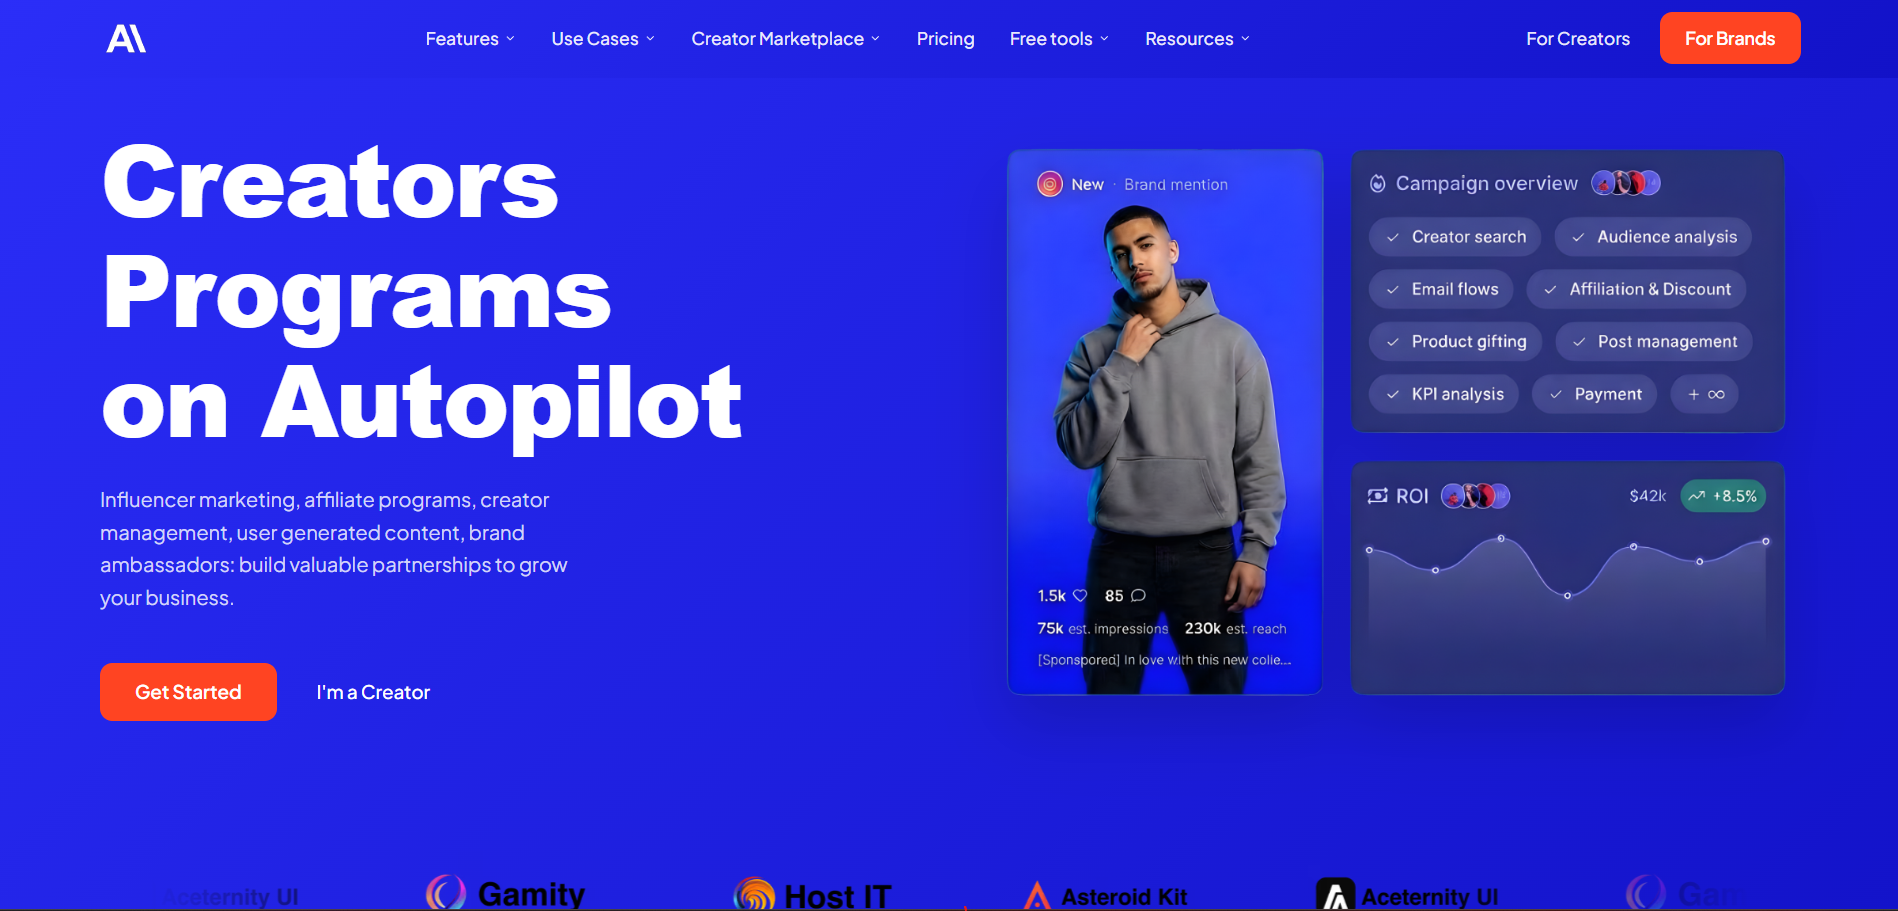
\includegraphics[width=0.9\textwidth]{screenshots/Screenshot 2026-06-10 120425.png}
    \caption{Our Platform Landing Page}
    \label{fig:usecase}
\end{figure}
\subsection{Brand Registration :}
This interface is used by companies to create a new account on our platform by providing basic information such as the company name, email address, website, and login credentials. Once the registration process is completed, brands can access the platform and start searching for influencers, creating campaigns, and managing collaborations.

\begin{figure}[H]
    \centering
    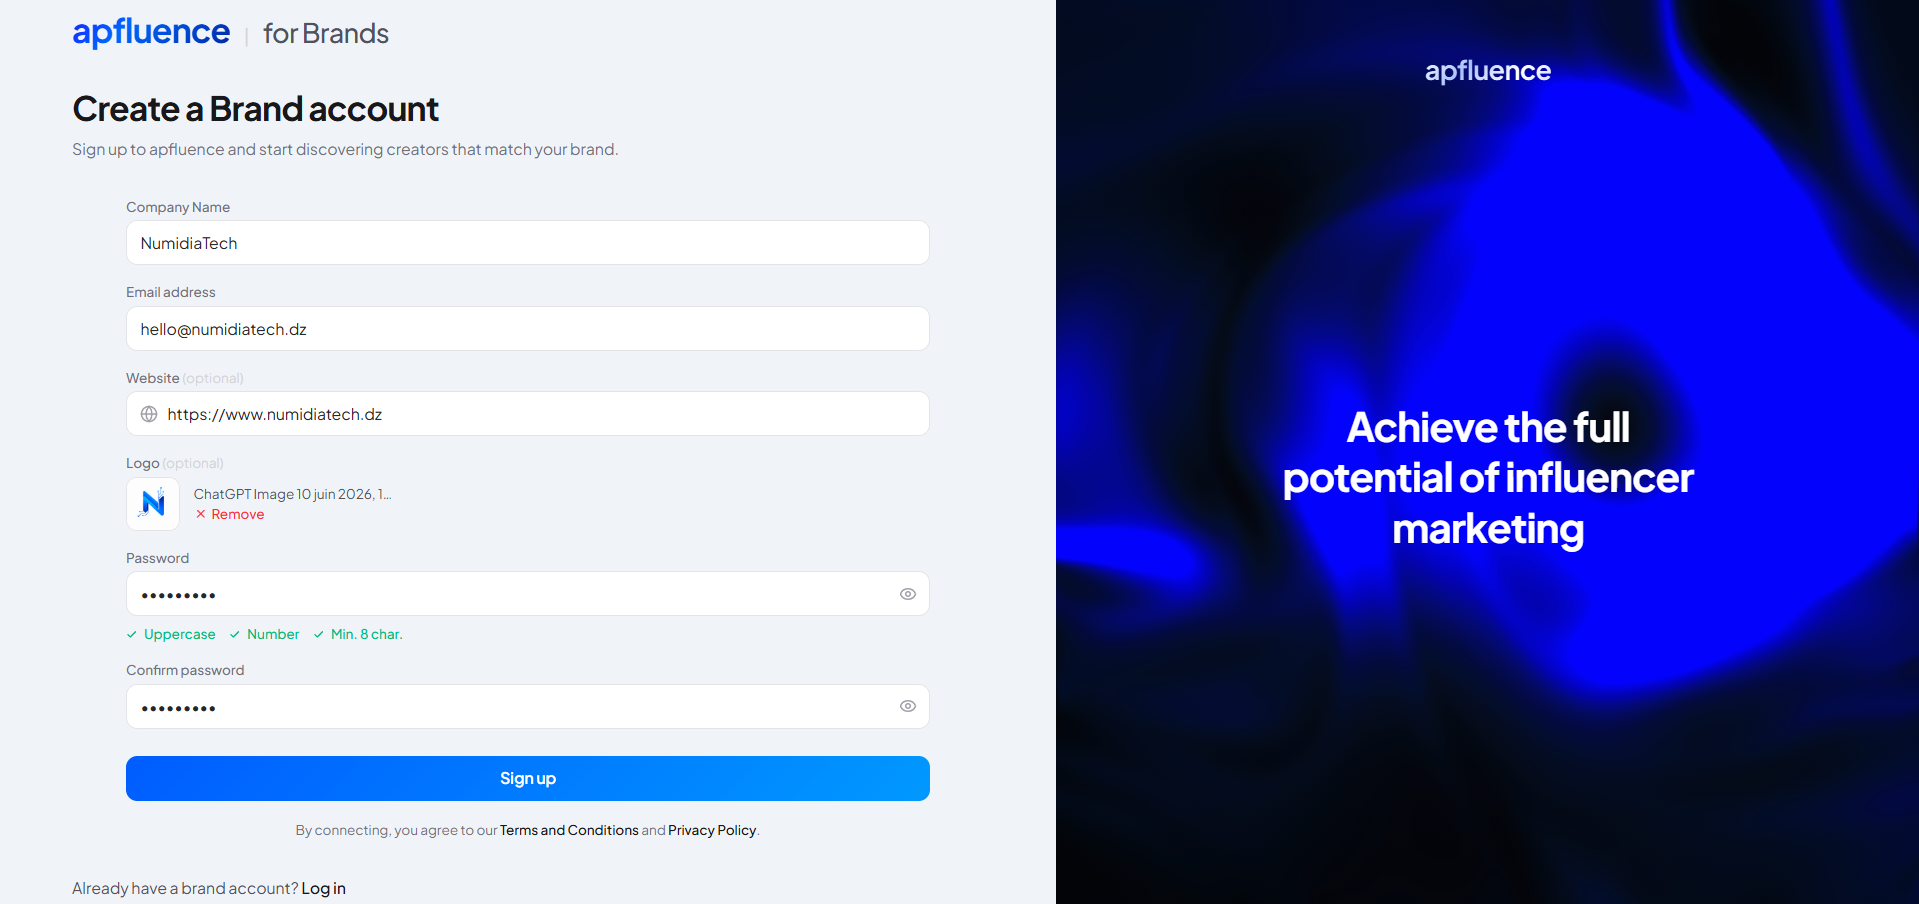
\includegraphics[width=0.9\textwidth]{screenshots/Screenshot 2026-06-10 124121.png}
    \caption{brand Registration interface}
    \label{fig:screenshot 1}
    \end{figure}
\begin{figure}[H]
    \centering
    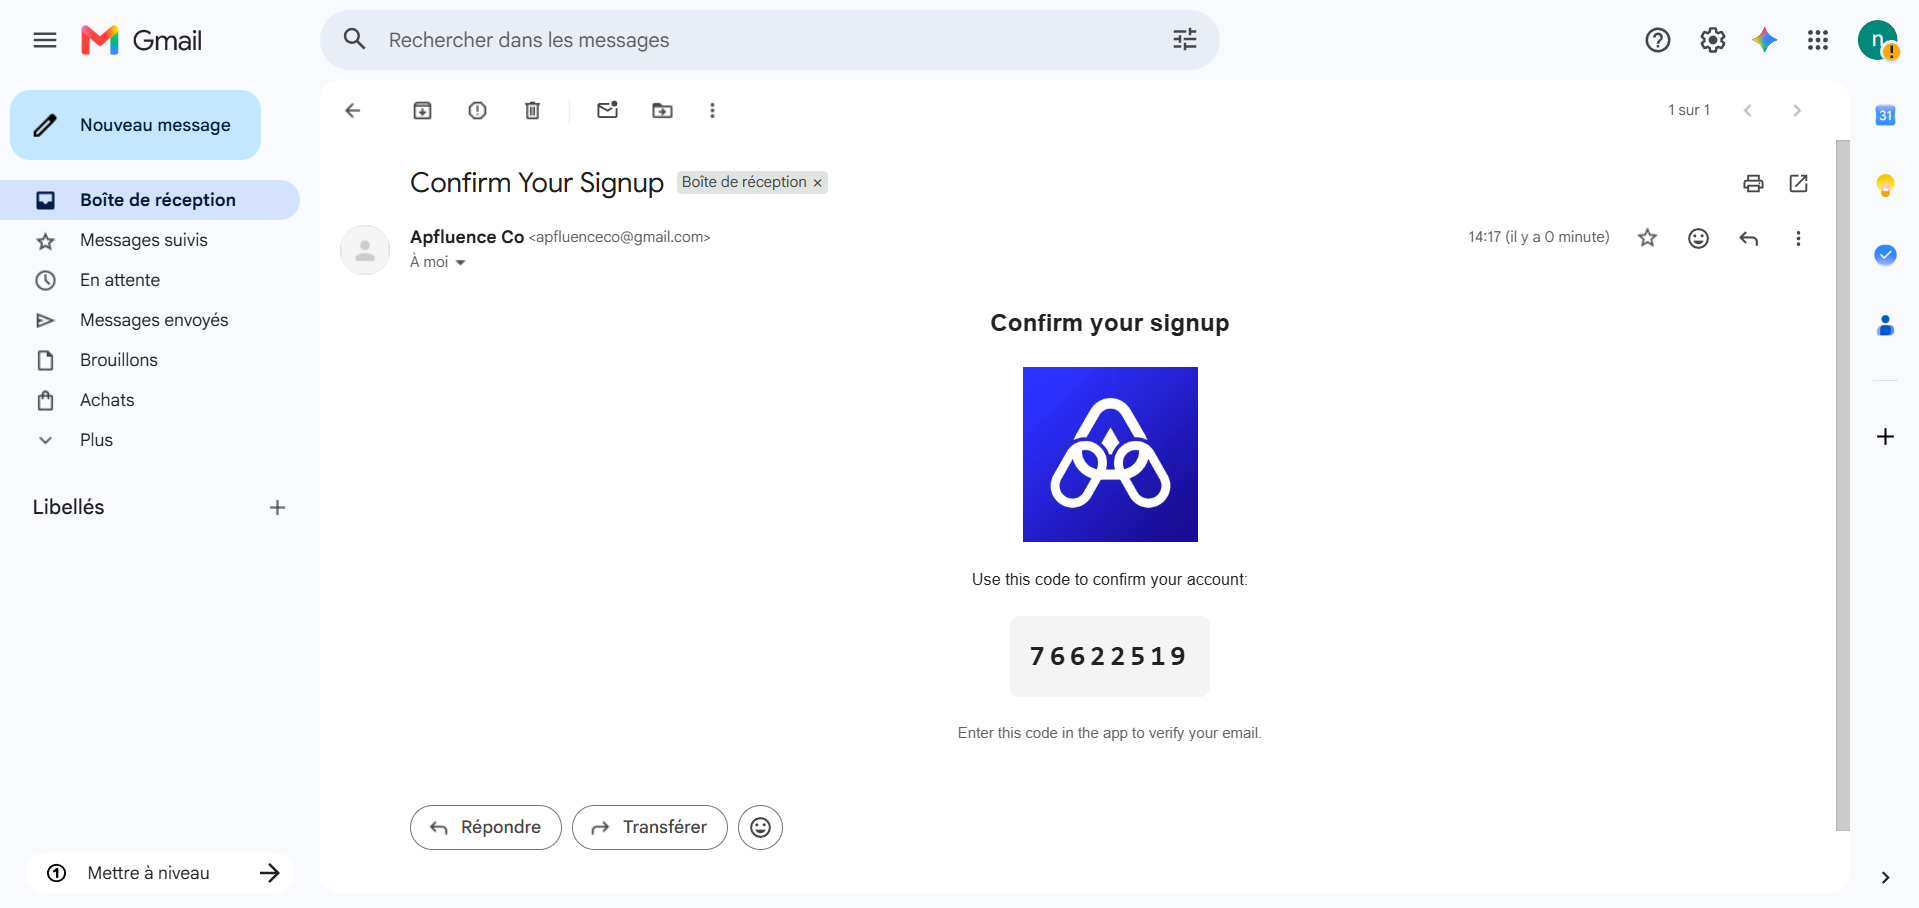
\includegraphics[width=0.9\textwidth]{screenshots/Screenshot 2026-06-10 141934.png}
    \caption{verfication code}
    \label{fig:screenshot 2}
\end{figure}
\subsection{Brand Dashboard Interface:}
\begin{figure}[H]
    \centering
    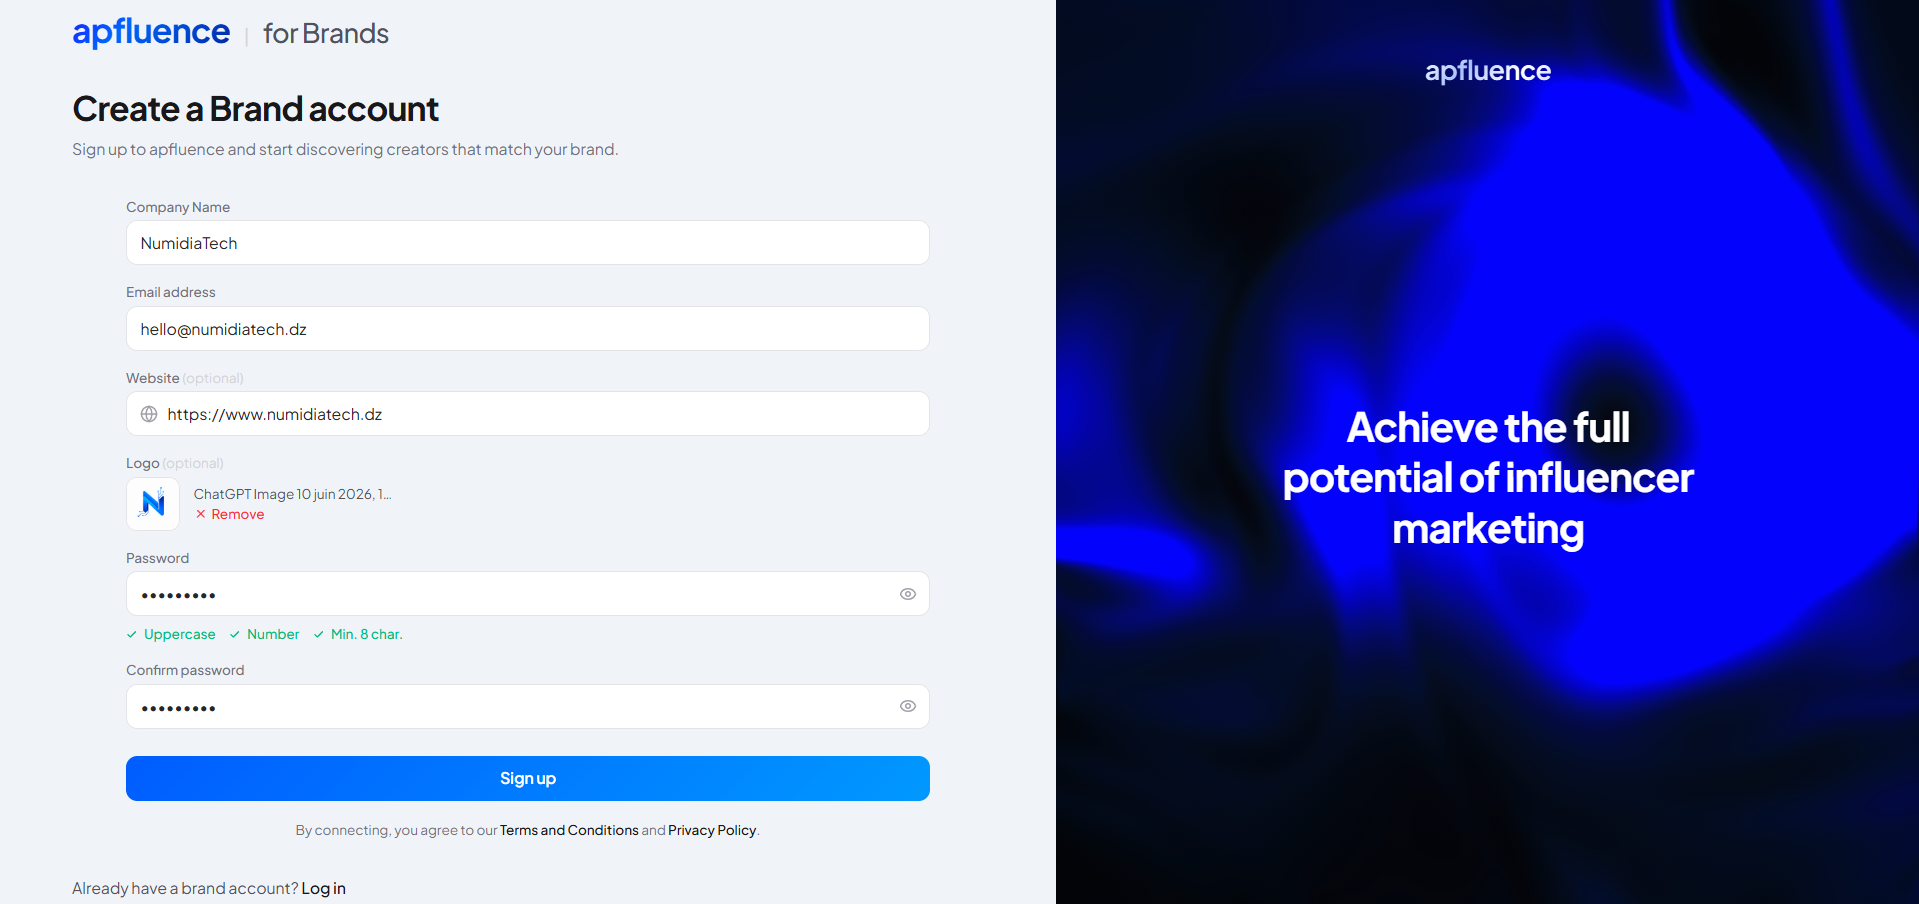
\includegraphics[width=0.9\textwidth]{screenshots/Screenshot 2026-06-10 124121.png}
    \caption{brand dashboard}
    \label{fig:screenshot 3}
\end{figure}
\subsection{Influencer Discovery Interface:}
\begin{figure}[H]
    \centering
    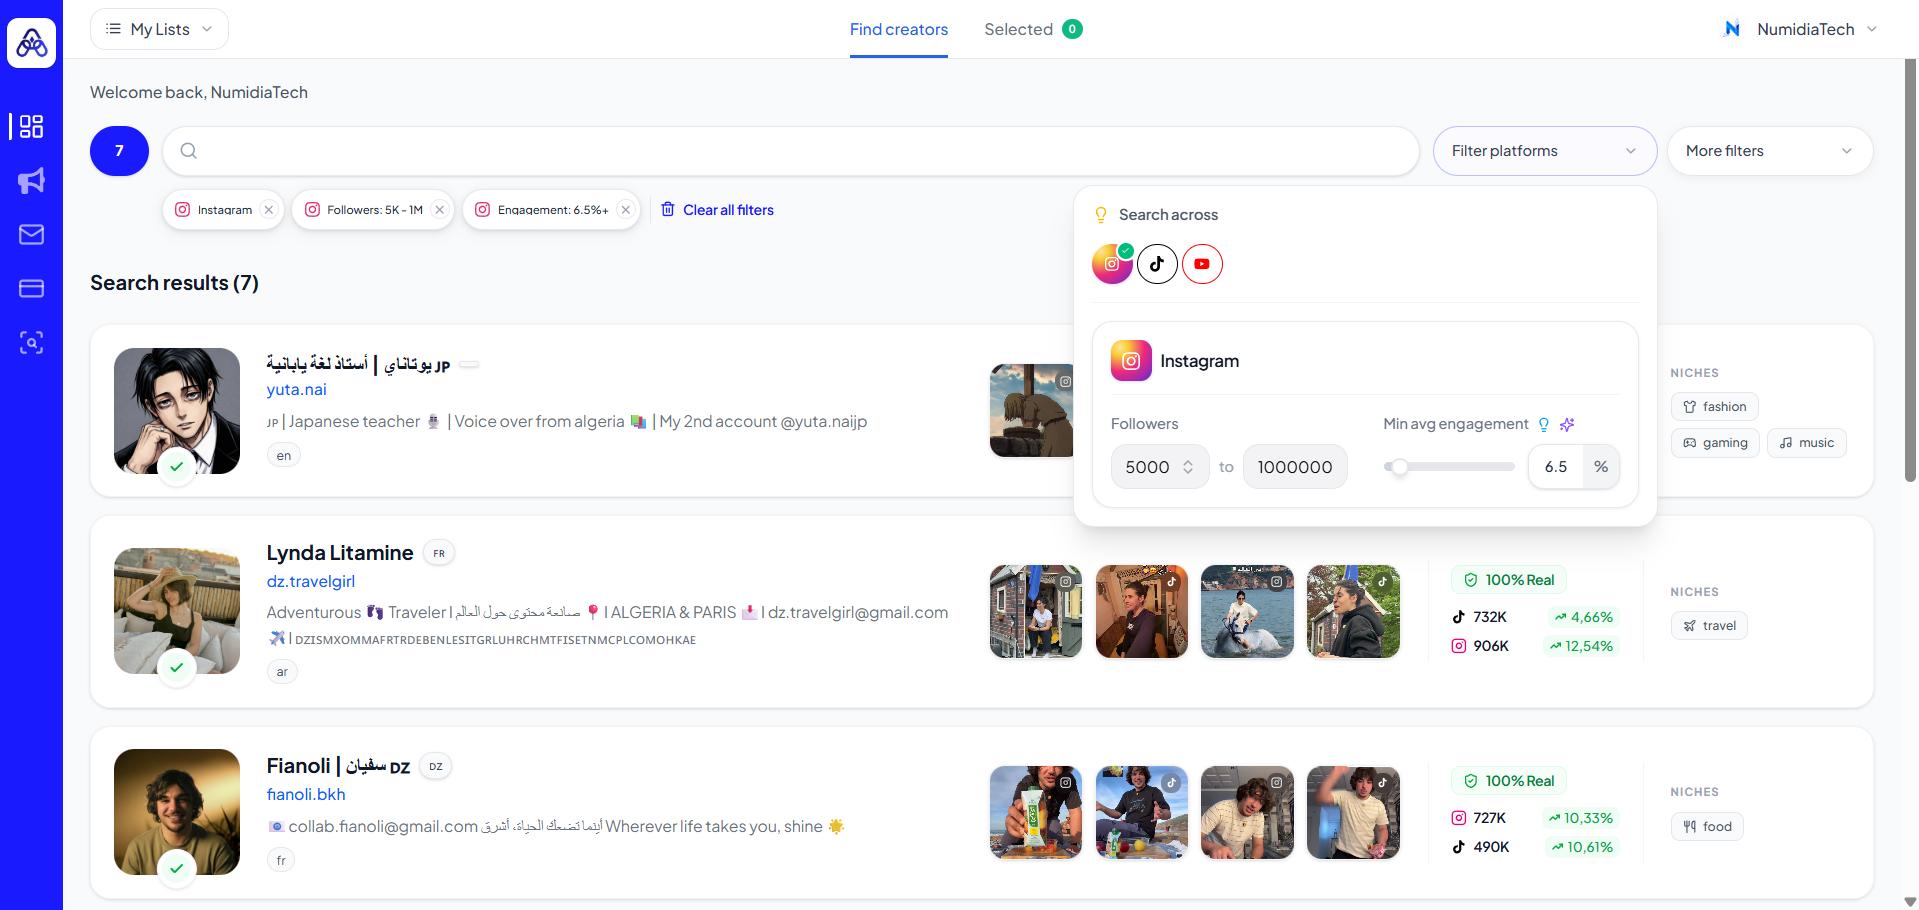
\includegraphics[width=0.9\textwidth]{screenshots/Screenshot 2026-06-10 143016.png}
    \caption{influencer discovery}
    \label{fig:screenshot 4}
\end{figure}

\subsection{Influencer Profile Interface:}
\begin{figure}[H]
    \centering
    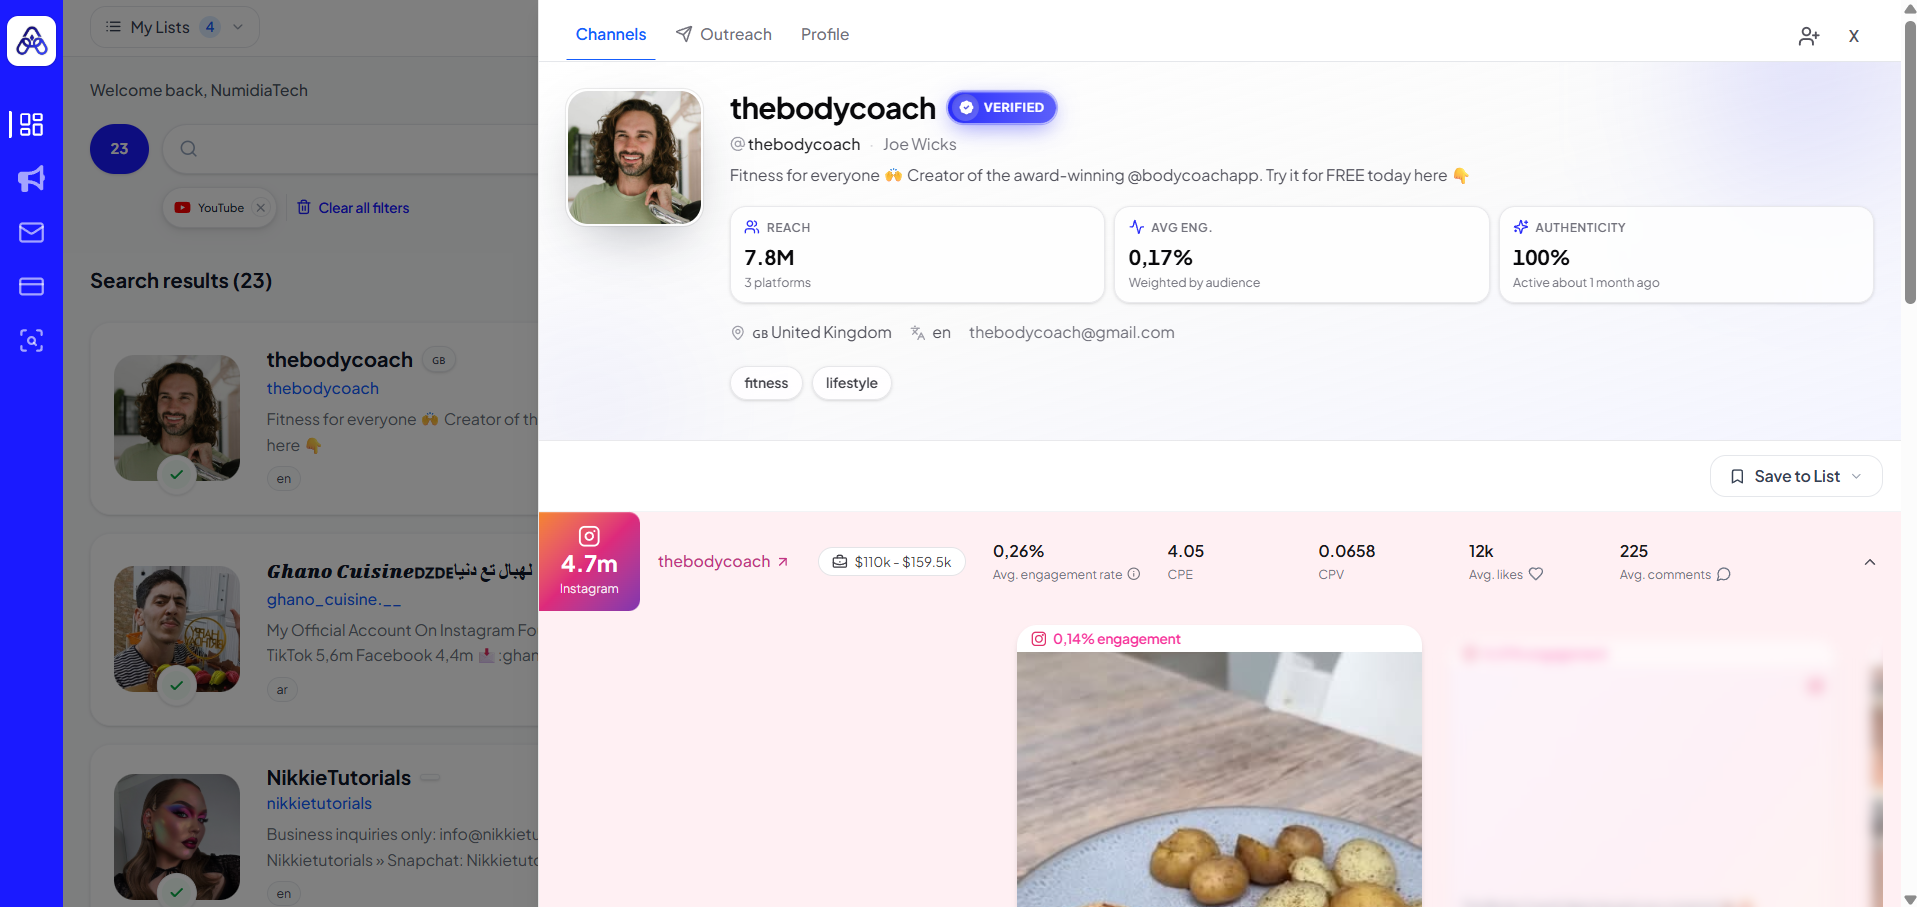
\includegraphics[width=0.9\textwidth]{screenshots/Screenshot 2026-06-10 143901.png}
    \caption{view  instagram influencer information}
    \label{fig:screenshot 5}
\end{figure}
\begin{figure}[H]
    \centering
    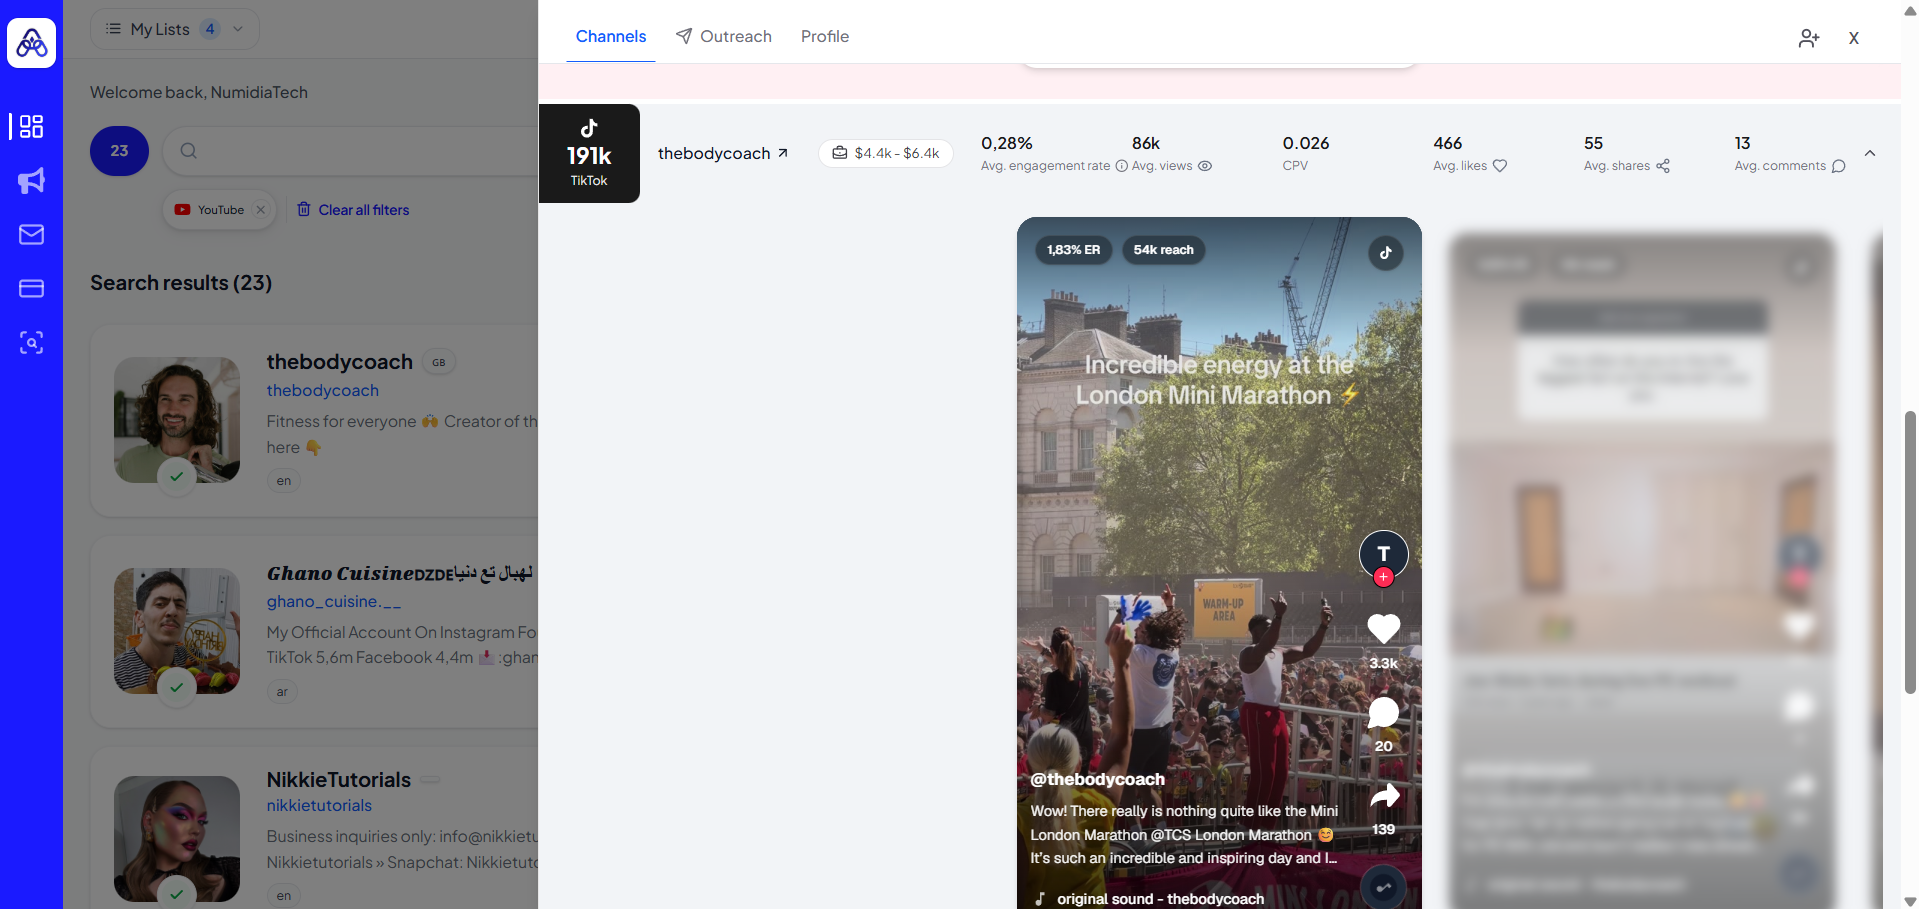
\includegraphics[width=0.9\textwidth]{screenshots/Screenshot 2026-06-10 144217.png}
    \caption{view tiktok influencer information}
    \label{fig:screenshot 6}
\end{figure}
\begin{figure}[H]
    \centering
    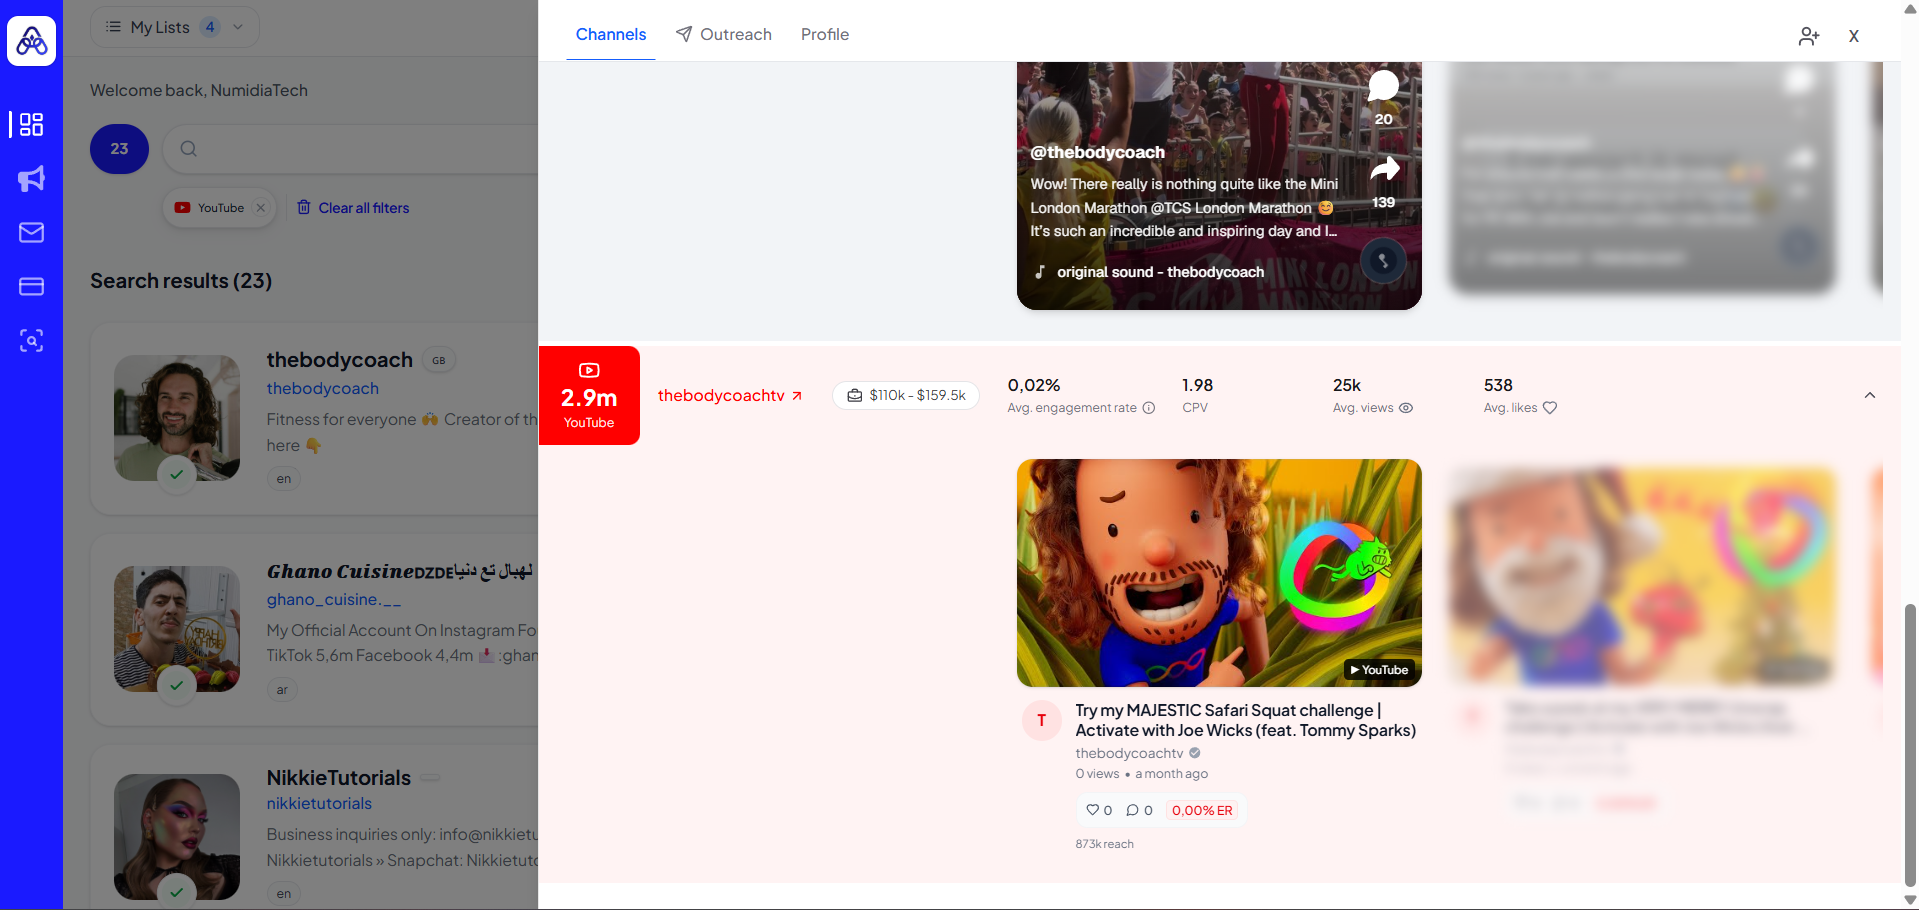
\includegraphics[width=0.9\textwidth]{screenshots/Screenshot 2026-06-10 144447.png}
    \caption{view youtube influencer information}
    \label{fig:screenshot 7}
\end{figure}
\subsection{Campaign Creation Interface:}
\begin{figure}[H]
    \centering
    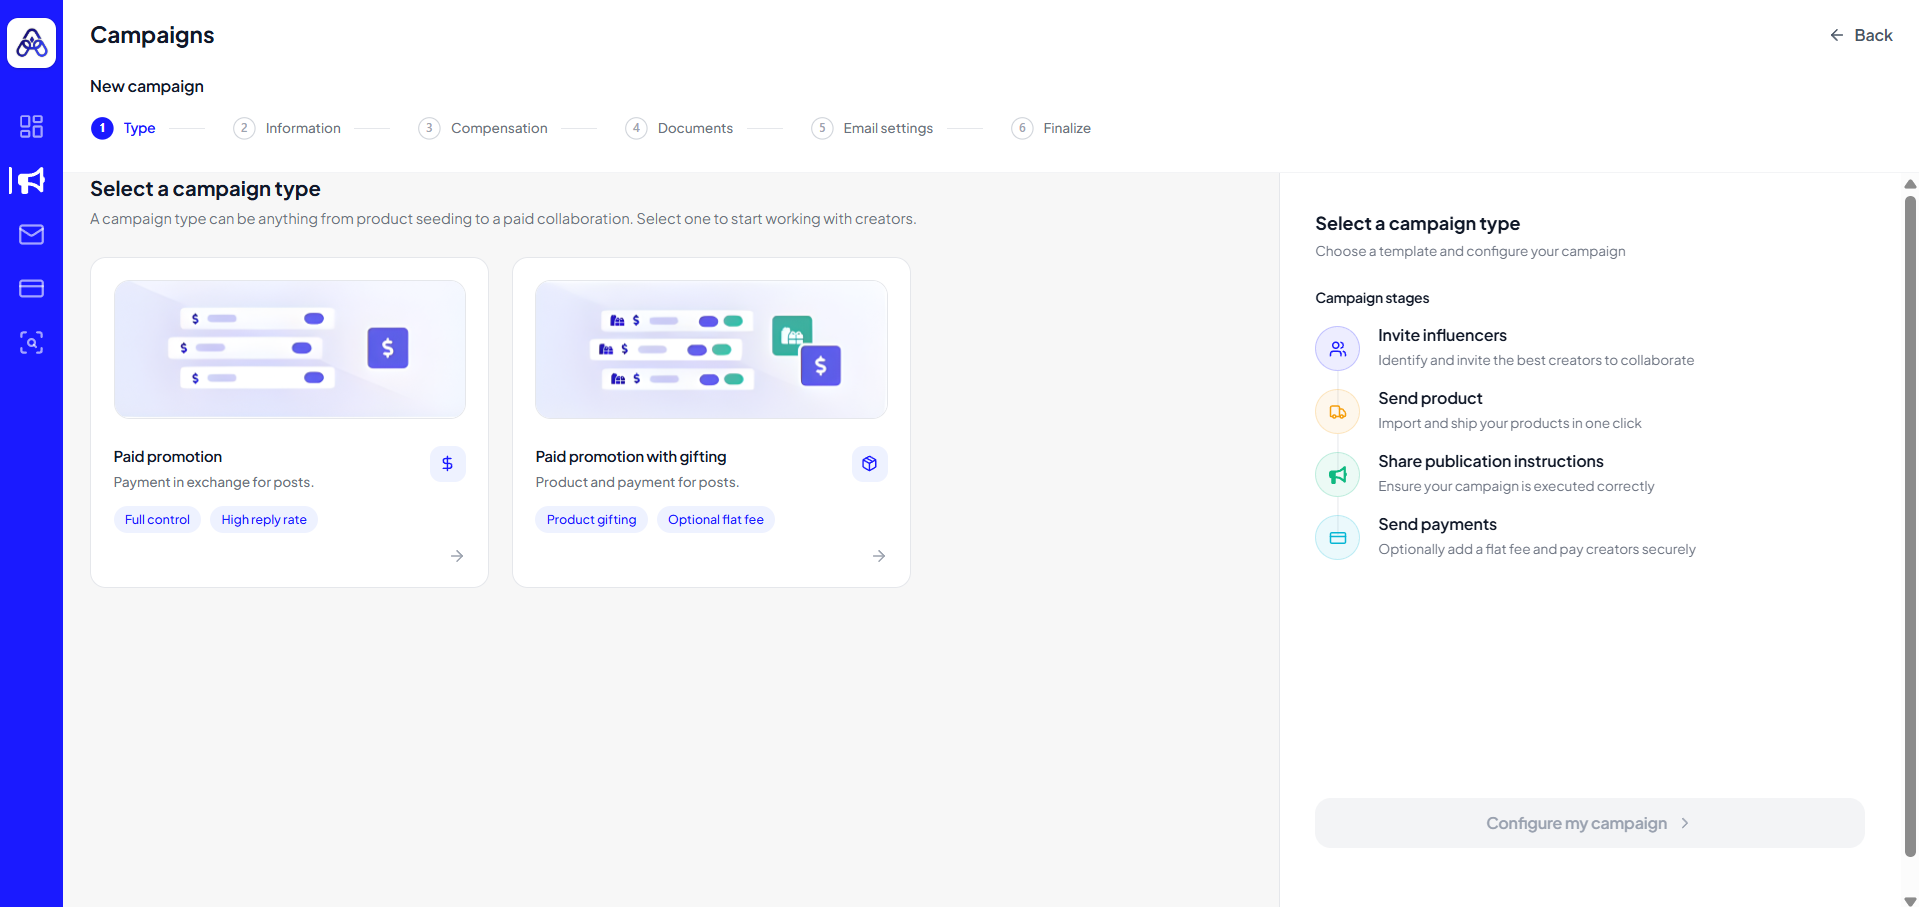
\includegraphics[width=0.9\textwidth]{screenshots/Screenshot 2026-06-10 155031.png}
    \caption{campaing type}
    \label{fig:screenshot 8}
\end{figure}
\begin{figure}[H]
    \centering
    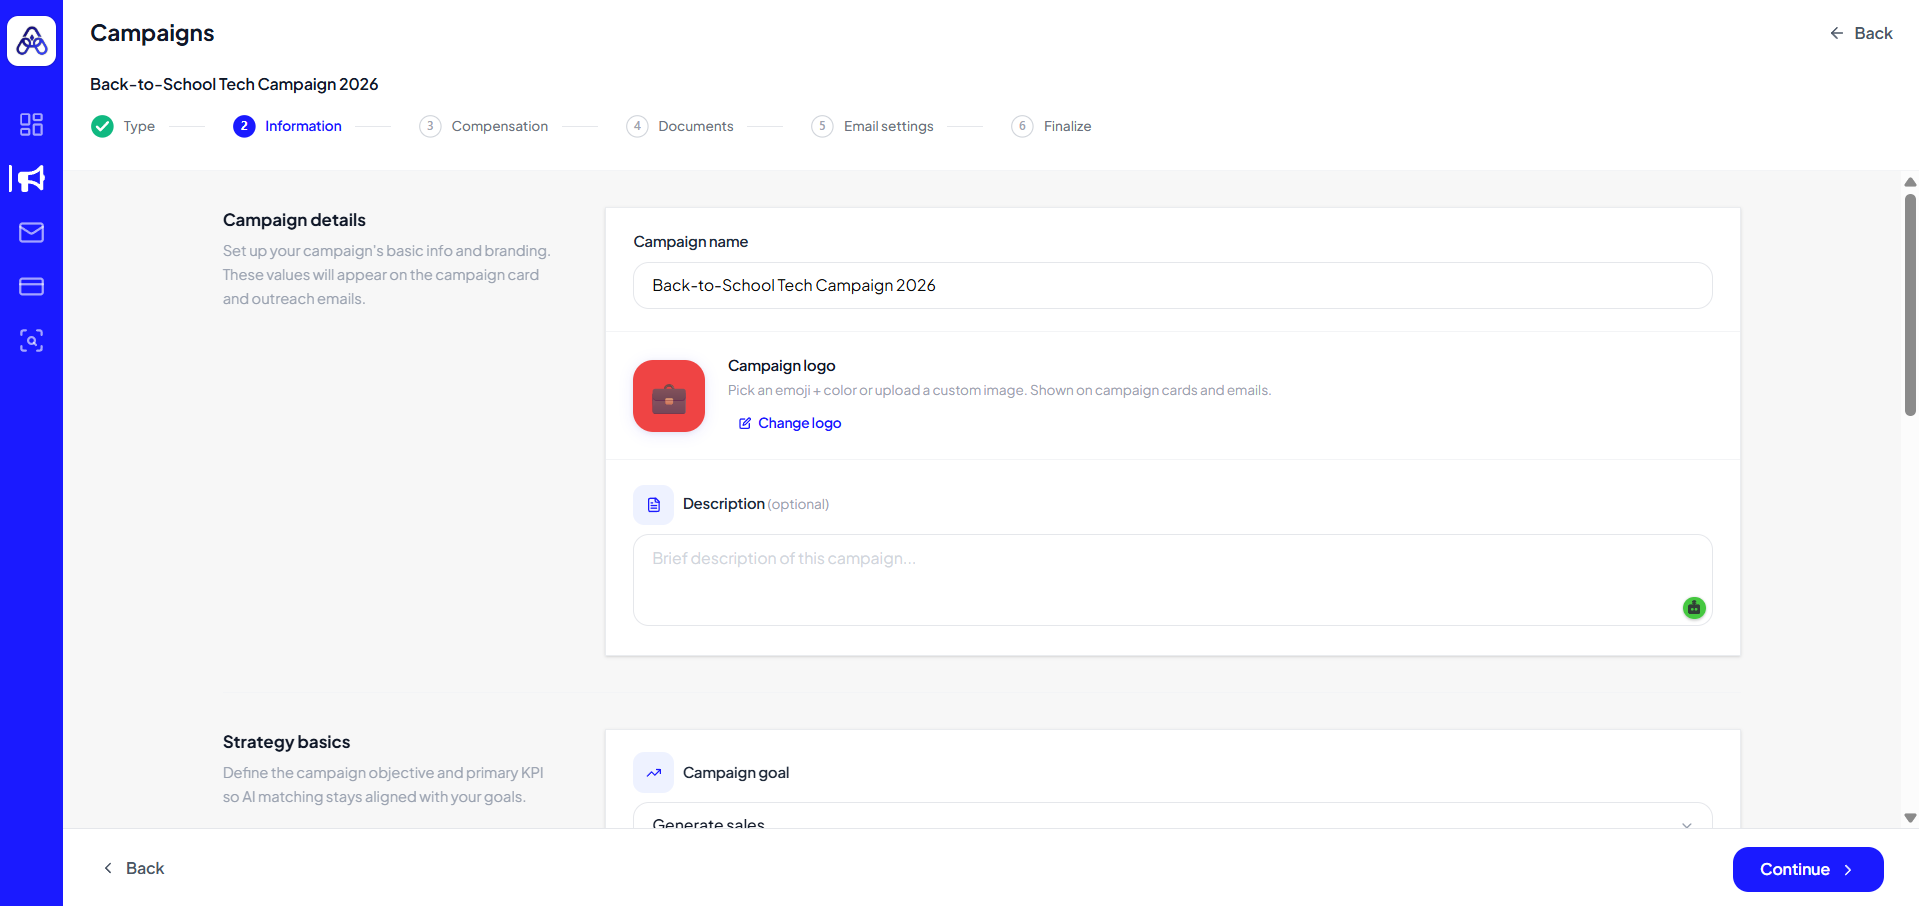
\includegraphics[width=0.9\textwidth]{screenshots/Screenshot 2026-06-10 155310.png}
    \caption{campaing  information part 1 }
    \label{fig:screenshot 9}
\end{figure}
\begin{figure}[H]
    \centering
    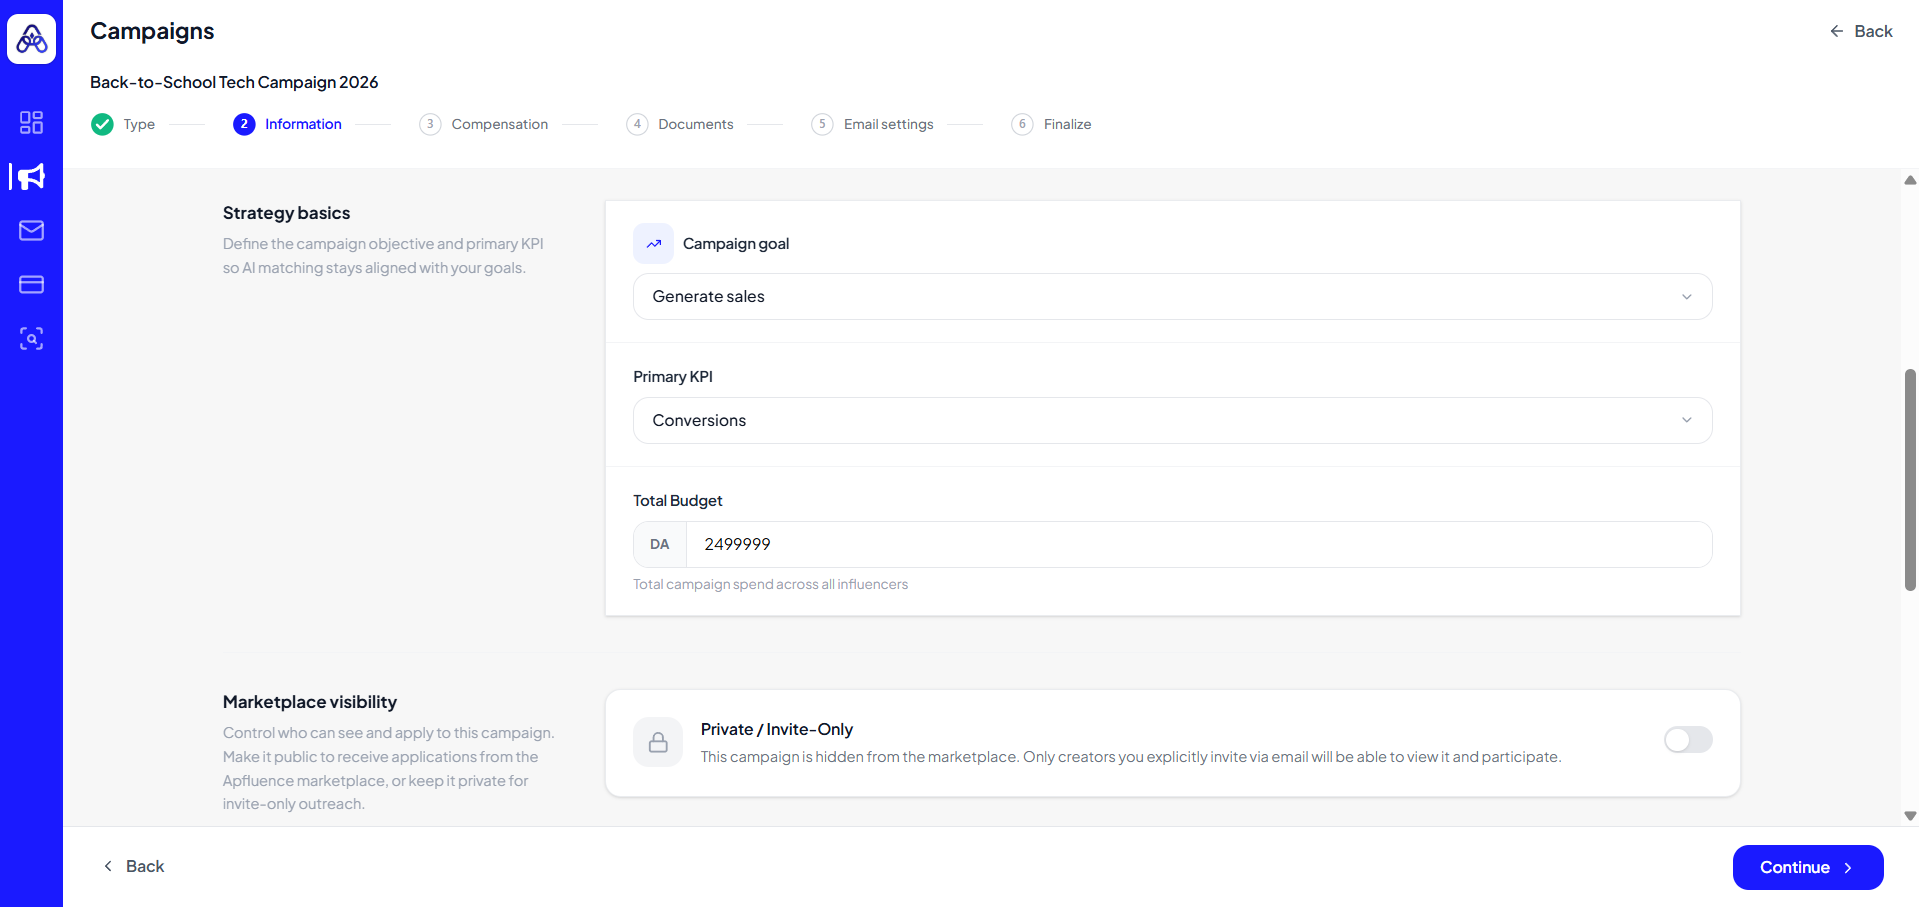
\includegraphics[width=0.9\textwidth]{screenshots/Screenshot 2026-06-10 155433.png}
    \caption{campaing  information part 2 }
    \label{fig:screenshot 9}
\end{figure}

\begin{figure}[H]
    \centering
    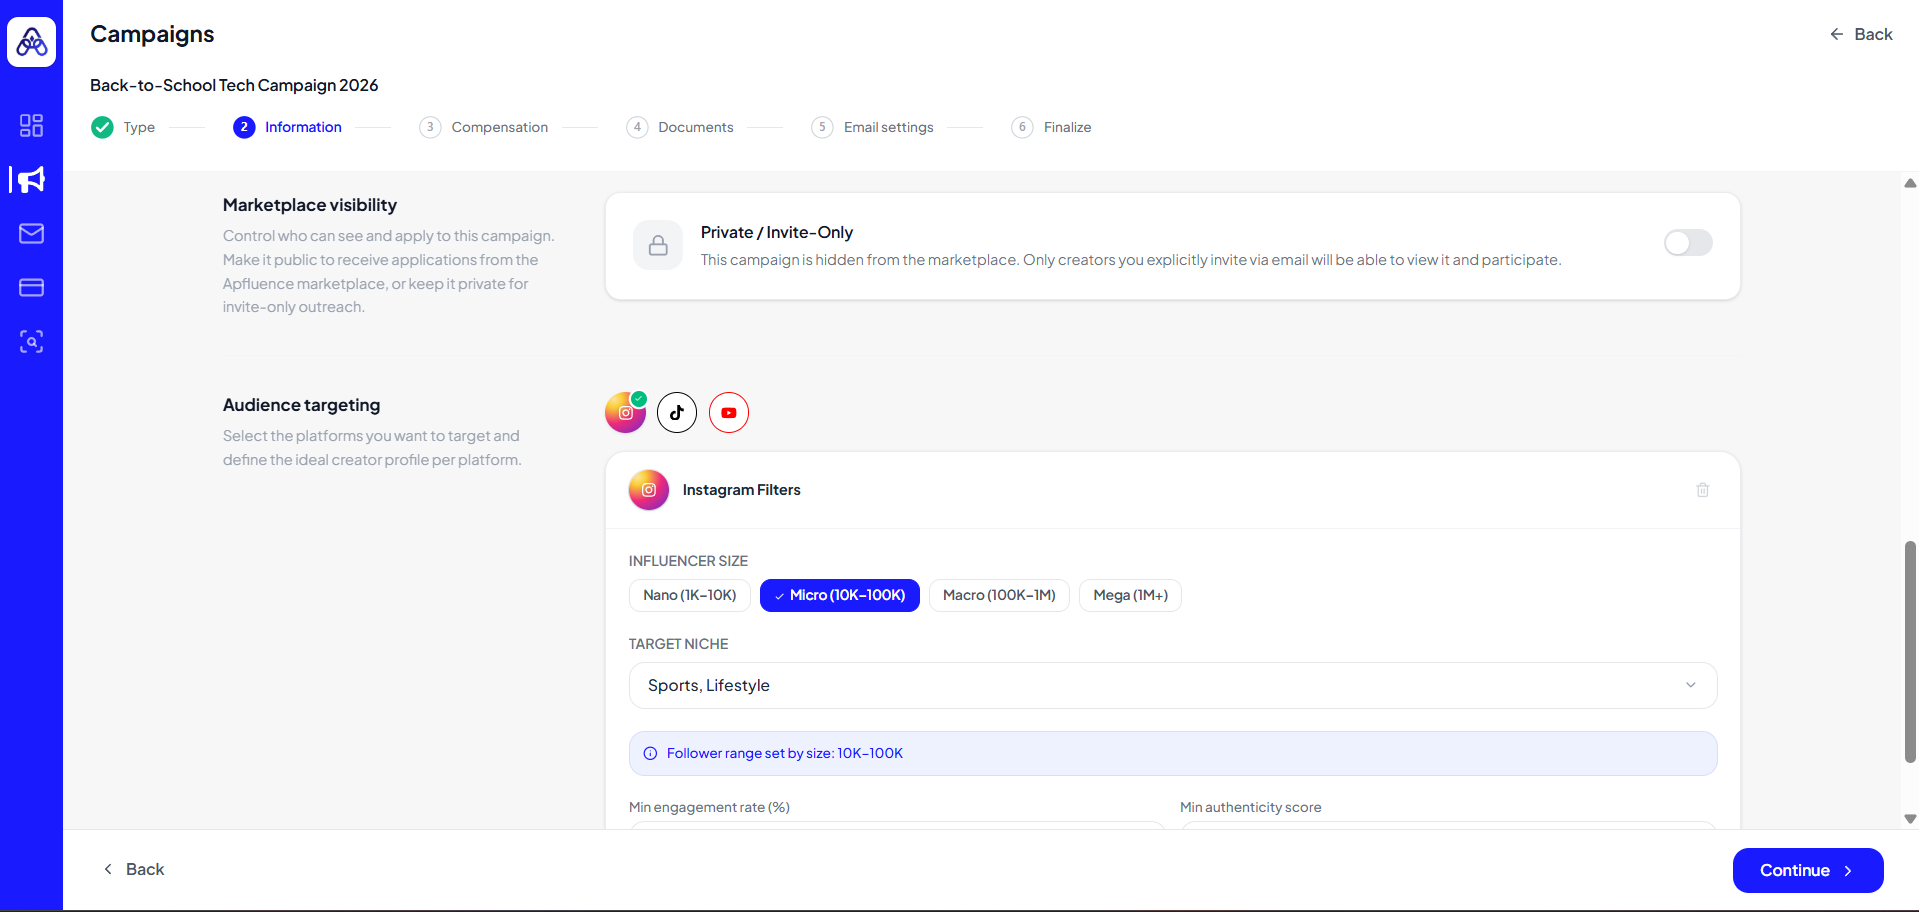
\includegraphics[width=0.9\textwidth]{screenshots/Screenshot 2026-06-10 155528.png}
    \caption{camping information part 3}
    \label{fig:screenshot 10}
\end{figure}


\begin{figure}[H]
    \centering
    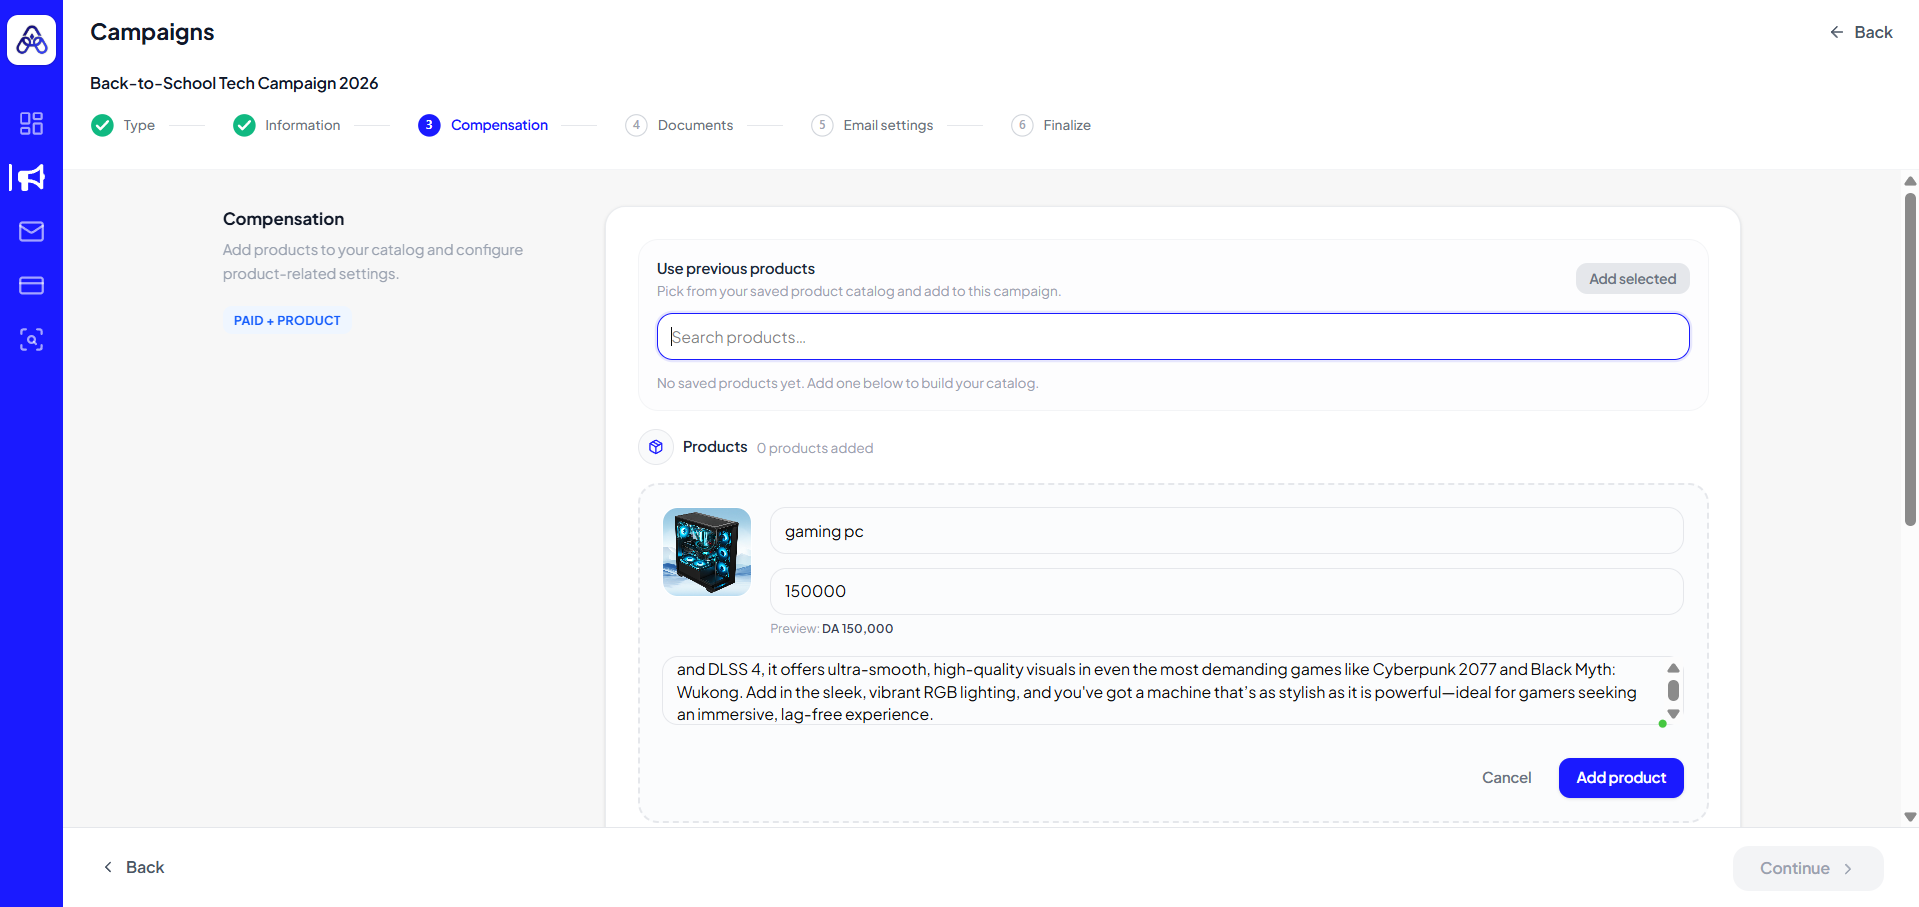
\includegraphics[width=0.9\textwidth]{screenshots/Screenshot 2026-06-10 155947.png}
    \caption{campaing product}
    \label{fig:screenshoot 11}
\end{figure}

\begin{figure}[H]
    \centering
    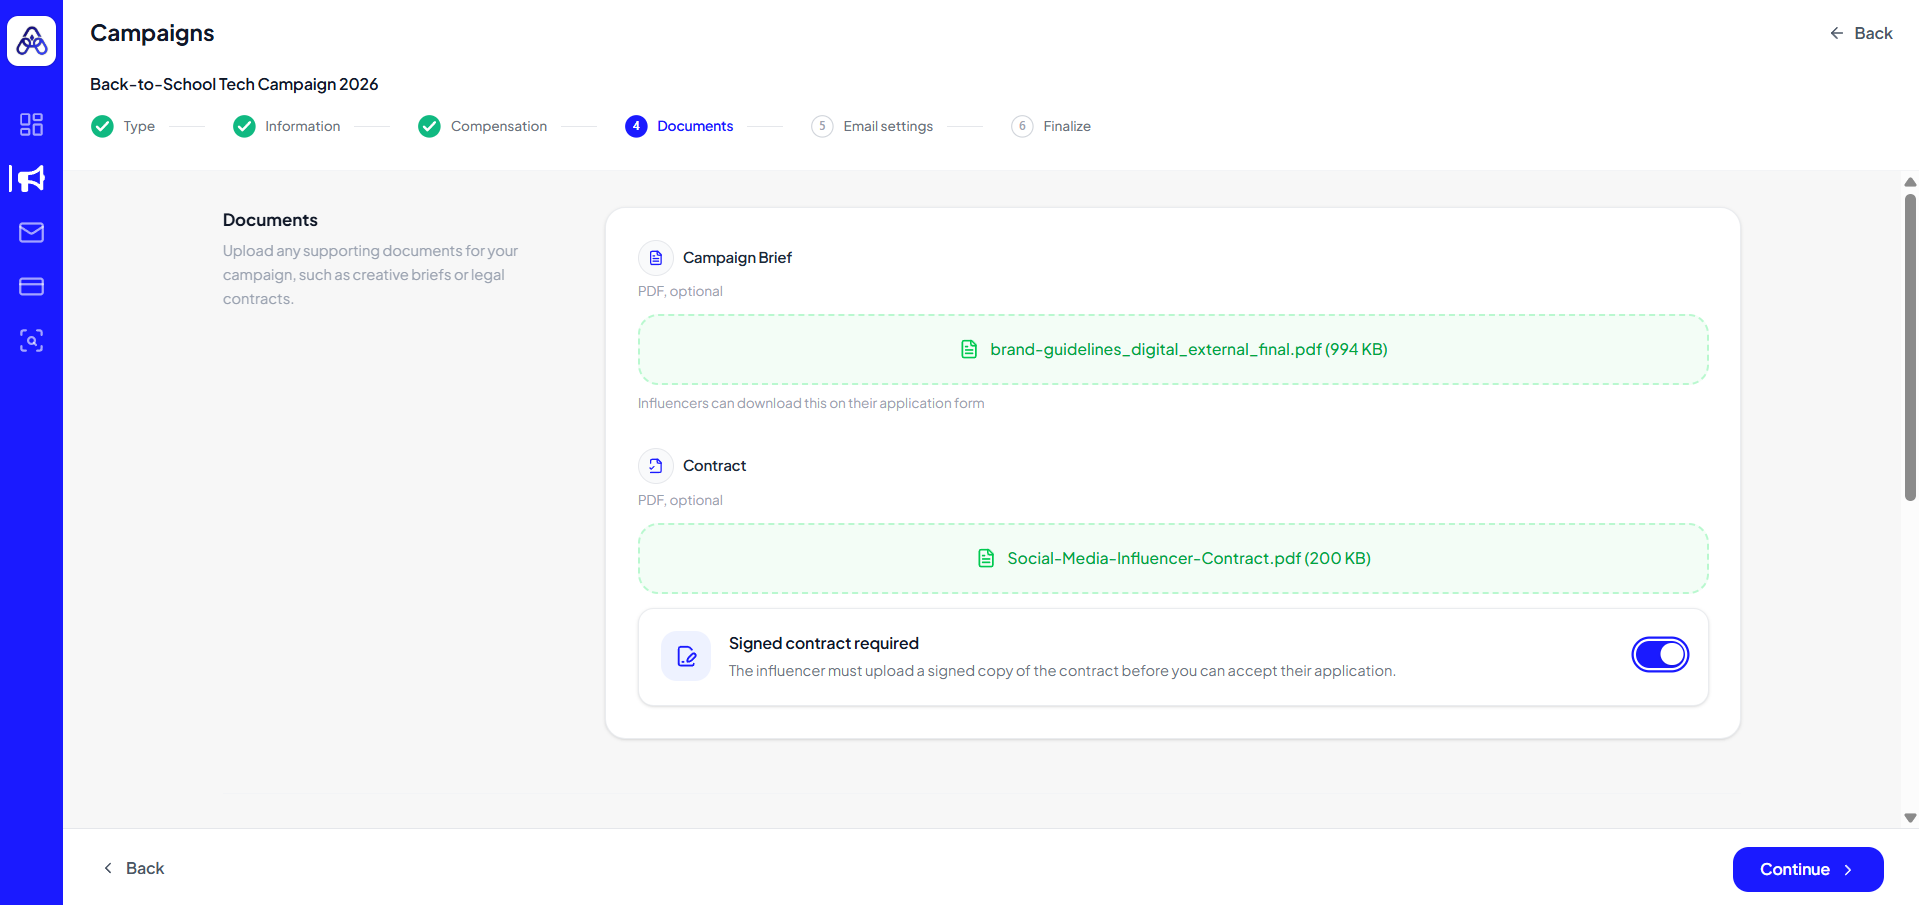
\includegraphics[width=0.9\textwidth]{screenshots/Screenshot 2026-06-10 163016.png}
    \caption{campaing documentation brief + contract}
    \label{fig:screenshoot 12}
\end{figure}
\begin{figure}[H]
    \centering
    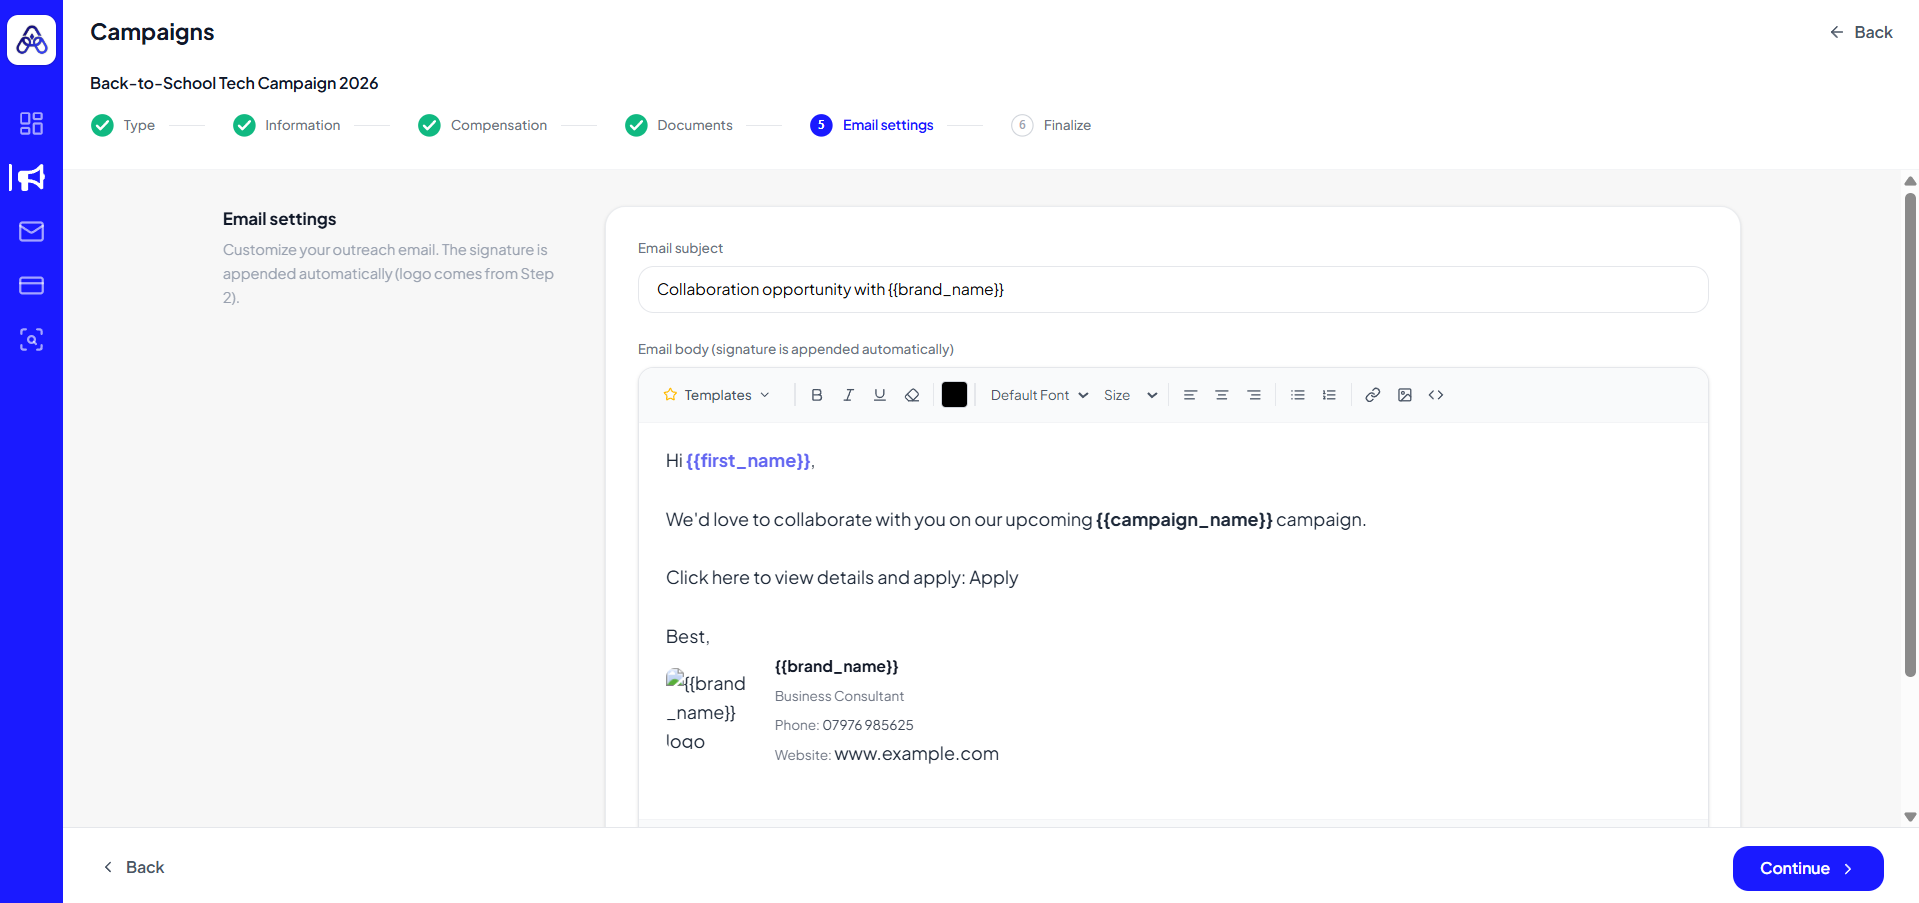
\includegraphics[width=0.9\textwidth]{screenshots/Screenshot 2026-06-10 163115.png}
    \caption{campaing outreach email}
    \label{fig:screenshoot 13}
\end{figure}
\begin{figure}[H]
    \centering
    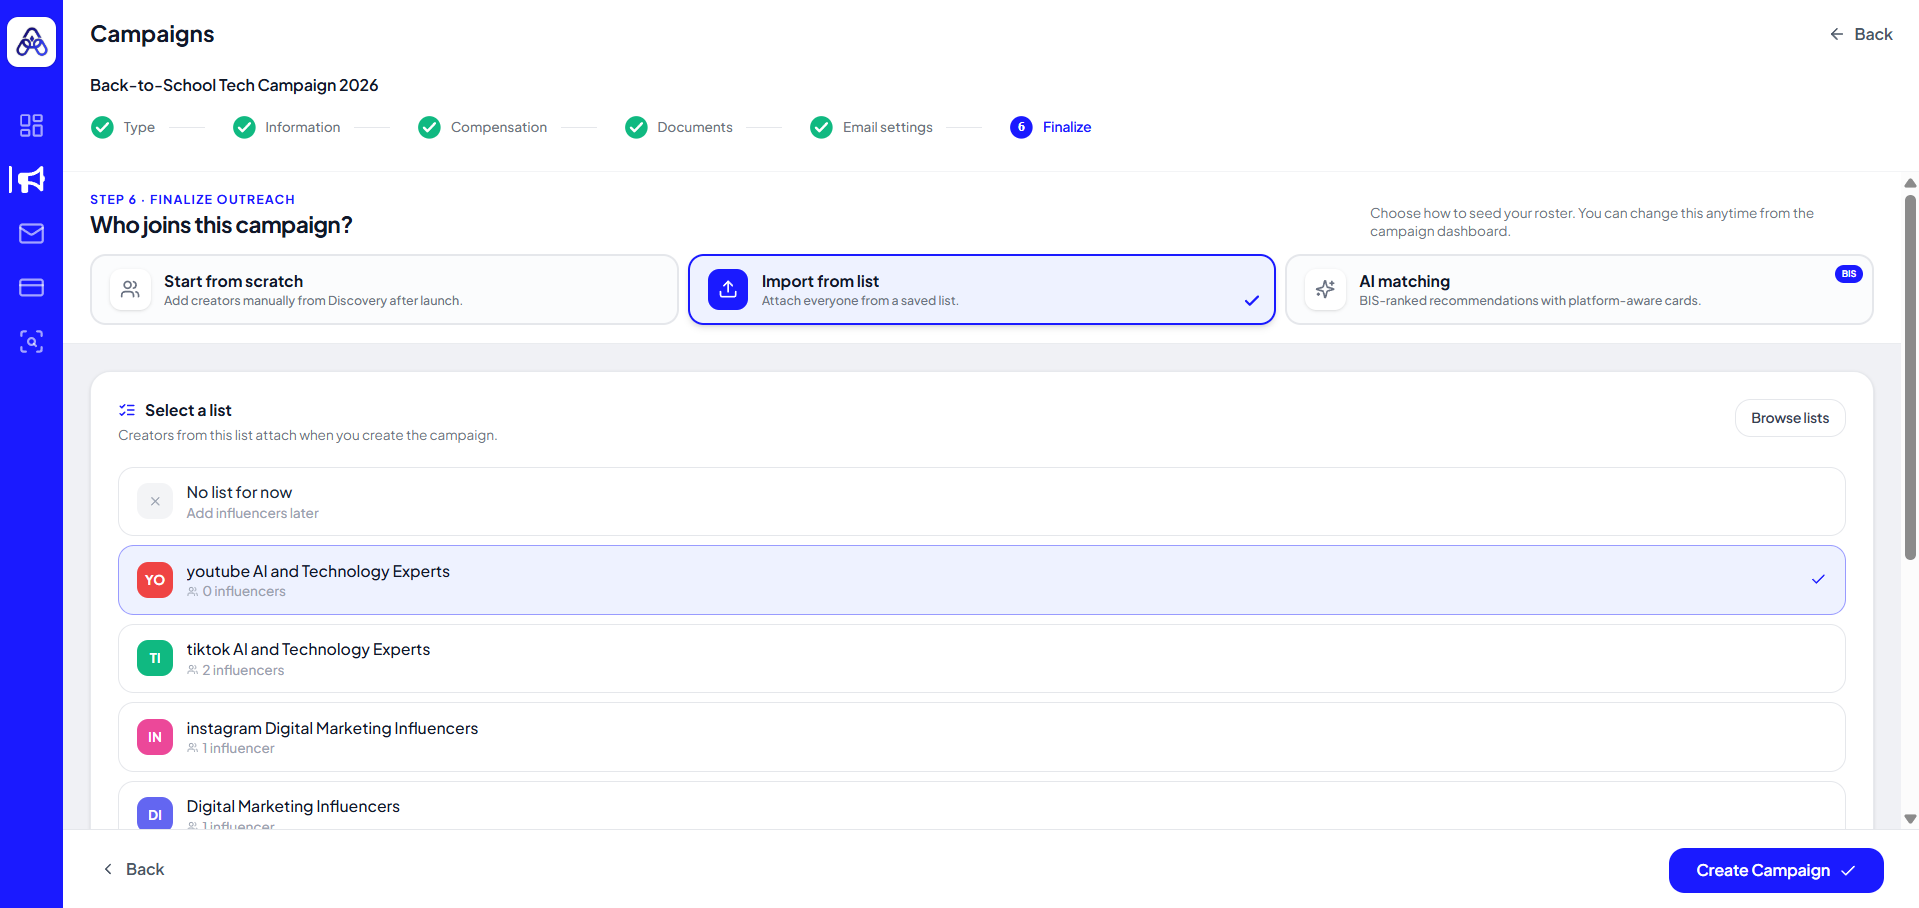
\includegraphics[width=0.9\textwidth]{screenshots/Screenshot 2026-06-10 164219.png}
    \caption{select list to campaing}
    \label{fig:screenshoot 14}
\end{figure}
\subsection{Campaign Management Interface:}
\begin{figure}[H]
    \centering
    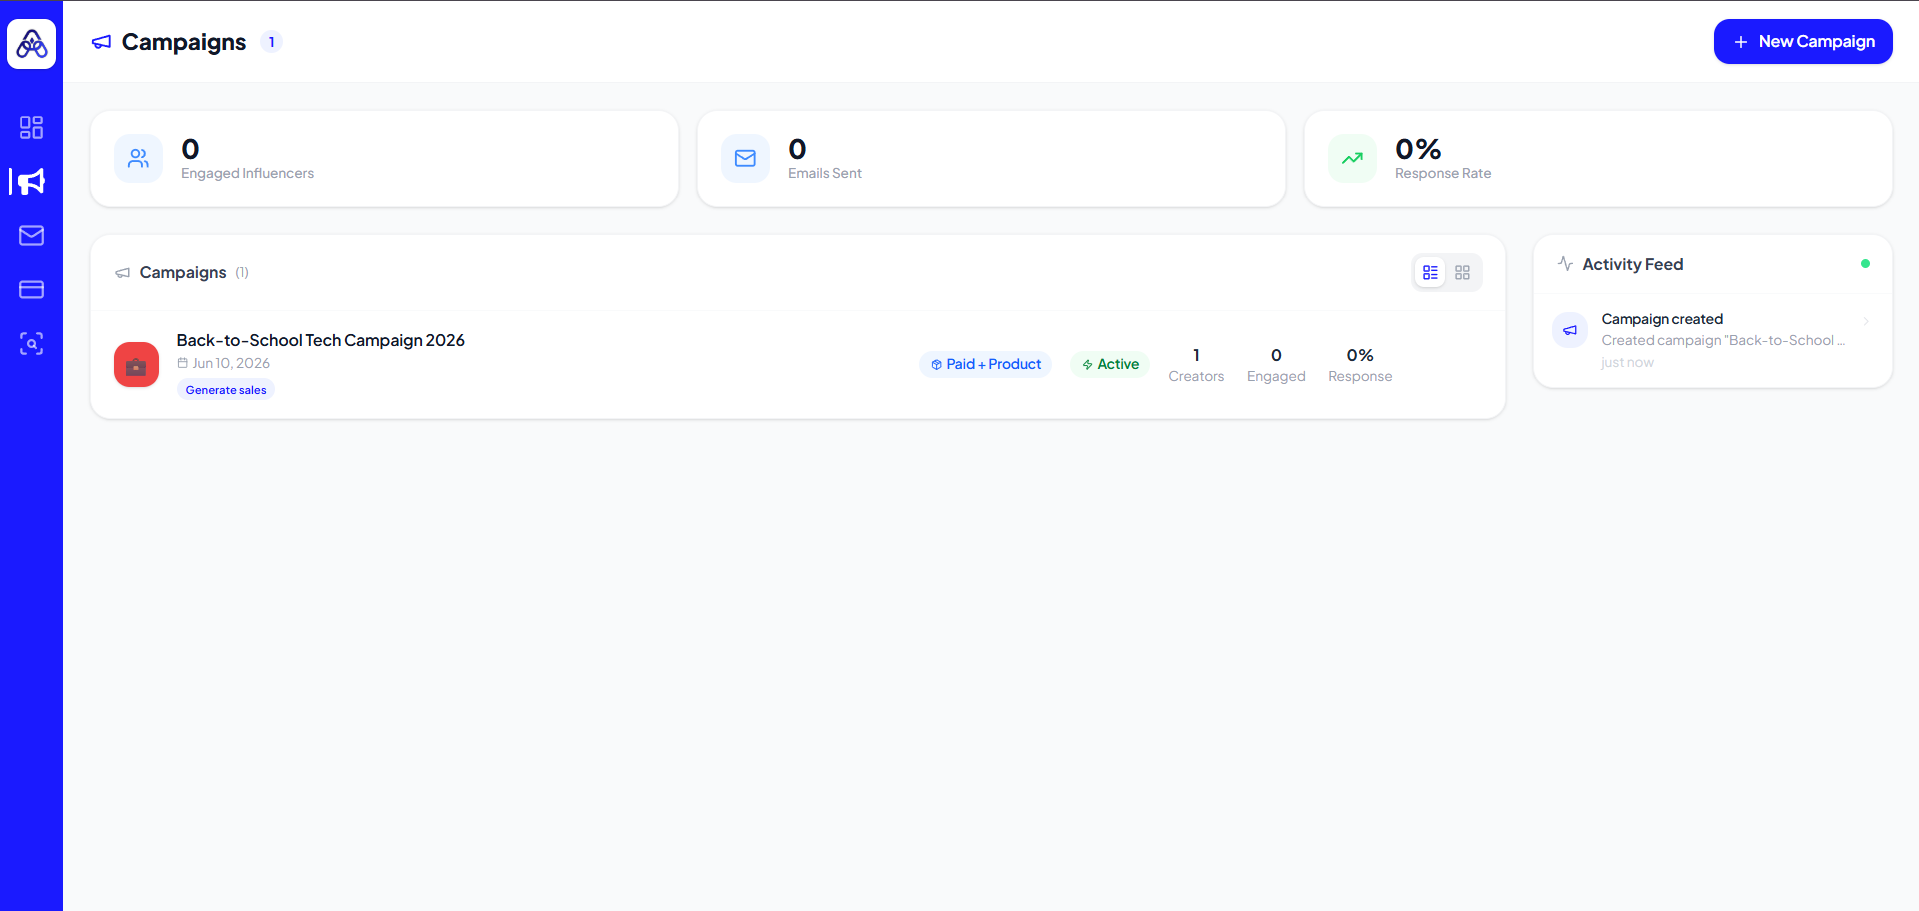
\includegraphics[width=0.9\textwidth]{screenshots/Screenshot 2026-06-10 164330.png}
    \caption{mange campaing}
    \label{fig:screenshoot 15}
\end{figure}
\begin{figure}[H]
    \centering
    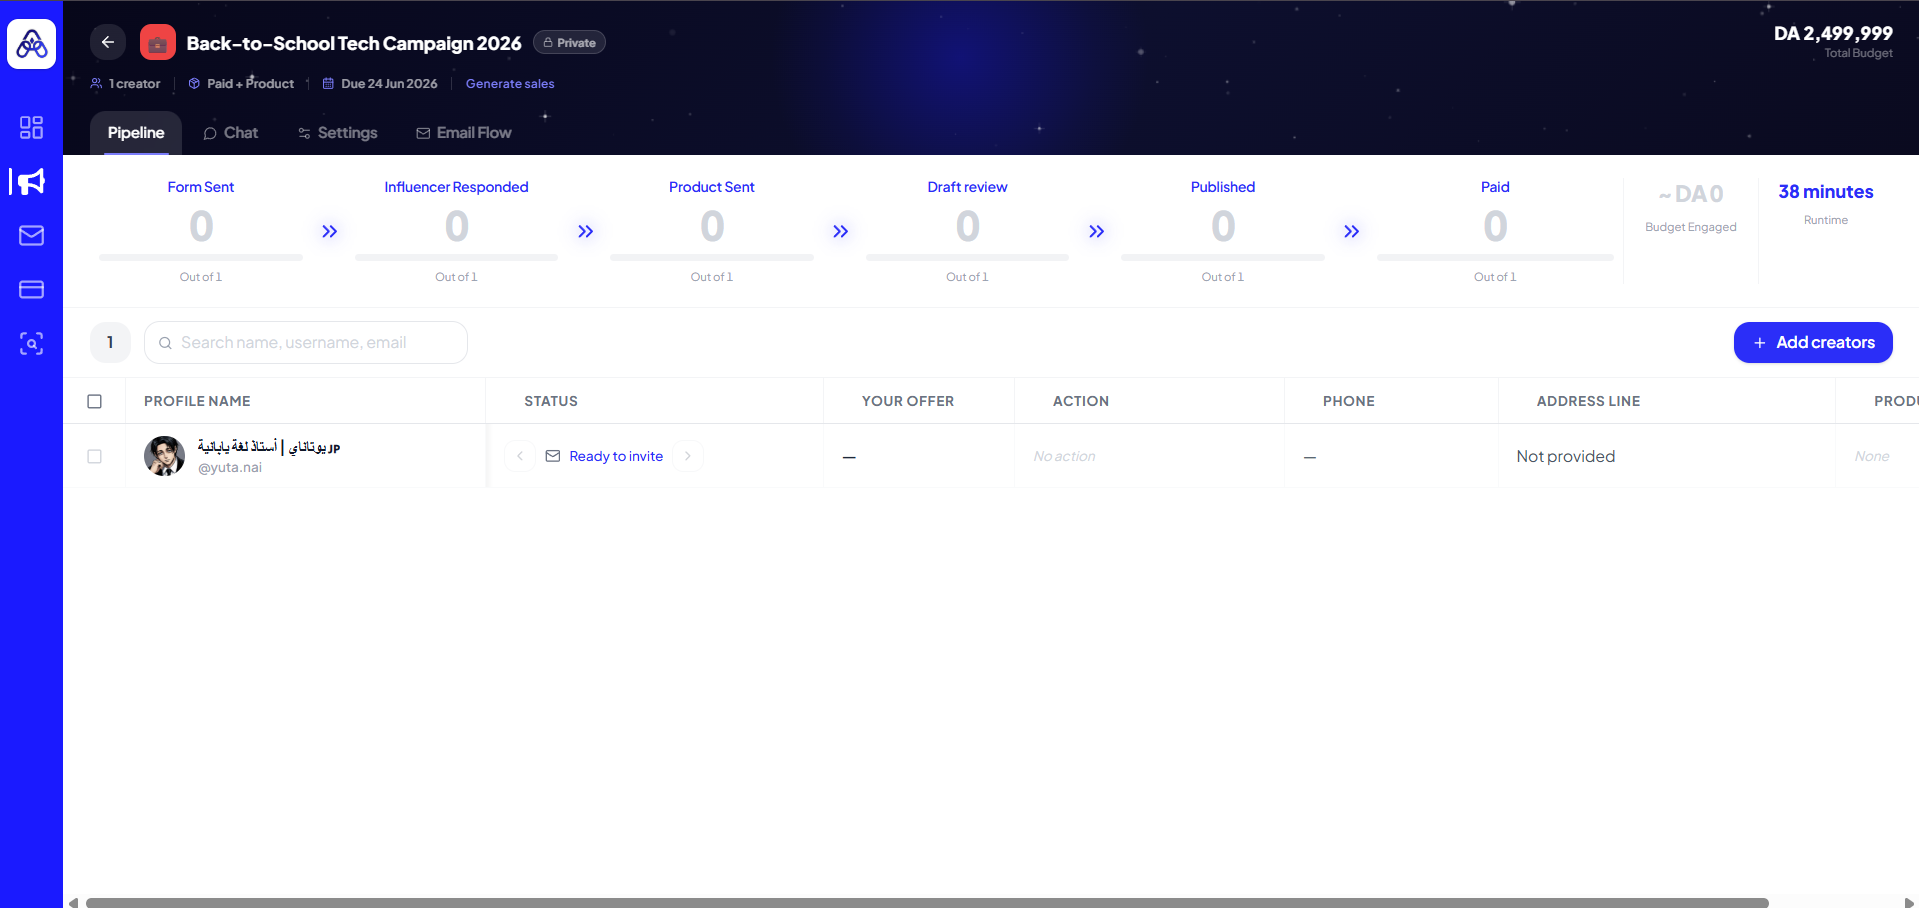
\includegraphics[width=0.9\textwidth]{screenshots/Screenshot 2026-06-10 172243.png}
    \caption{mange campaing}
    \label{fig:screenshoot 16}
\end{figure}
\subsection{Communication (chat):}
\begin{figure}[H]
    \centering
    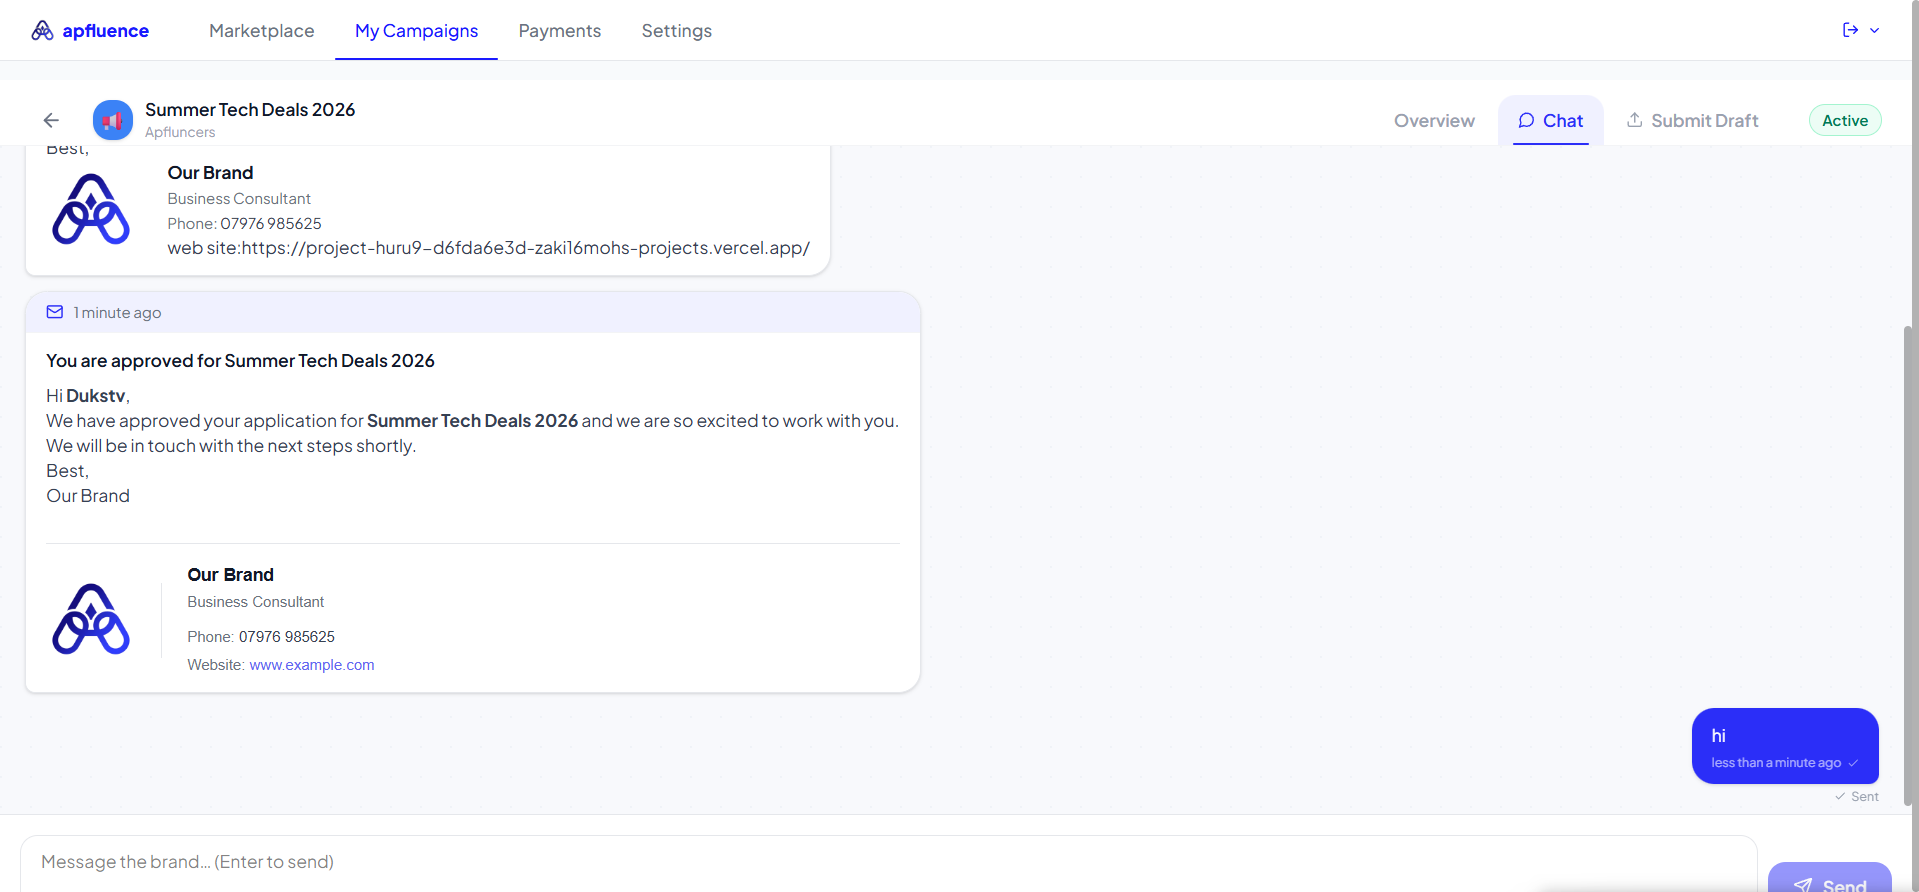
\includegraphics[width=0.9\textwidth]{screenshots/Screenshot 2026-06-10 203351.png}
    \caption{chat infeluencer / brand}
    \label{fig:screenshoot 17}
\end{figure}
\subsection{Payment Management :}
\begin{figure}[H]
    \centering
    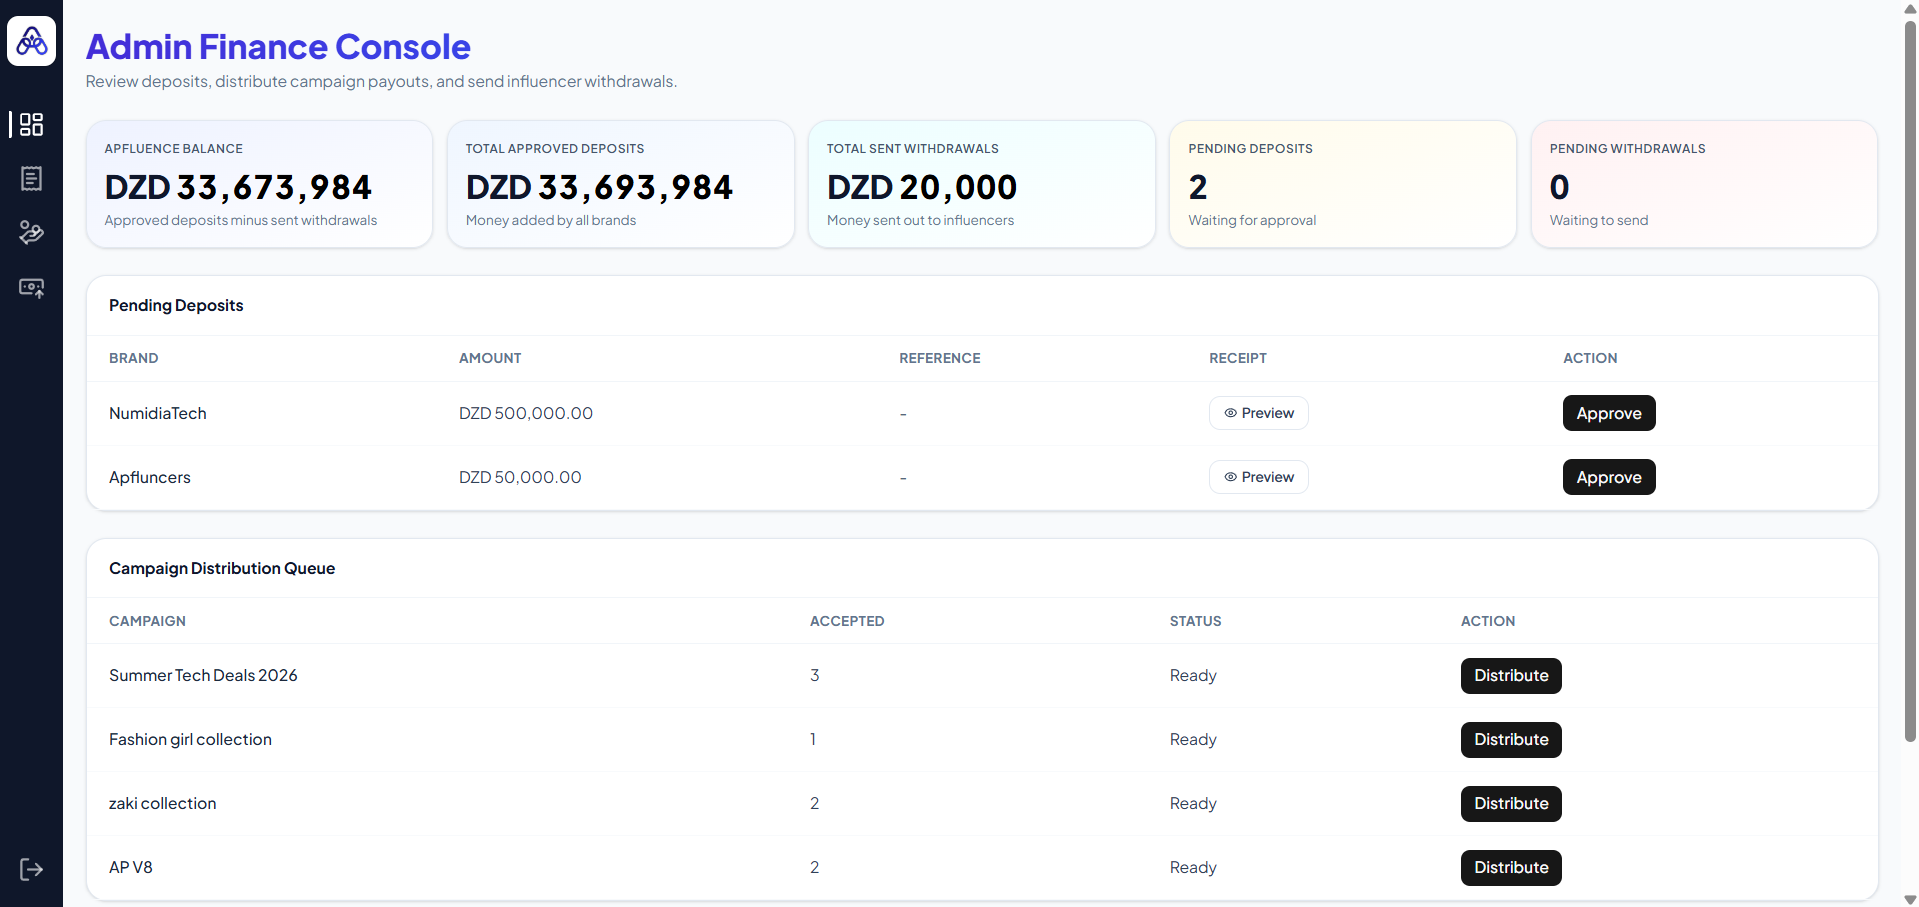
\includegraphics[width=0.9\textwidth]{screenshots/Screenshot 2026-06-10 204928.png}
    \caption{managment payment}
    \label{fig:screenshoot 18}
\end{figure}